\documentclass[10pt]{scrreprt}

% quick TOC setup
\KOMAoption{toc}{chapterentrydotfill}
% don't use parskip package, set parskip=full instead
\KOMAoption{parskip}{half}

\usepackage[twoside
            ,papersize={148mm, 210mm}
            ,layoutsize={148mm, 210mm}
            ,top=1.5cm
            ,bottom=2cm
            ,footskip=1cm
            ,textwidth=12cm
            ,verbose
            ]{geometry}

\renewcommand*{\chapterheadstartvskip}{}

\usepackage[parfill]{parskip}
\usepackage{graphicx}
\usepackage{fancyhdr}
\usepackage{eso-pic}
\usepackage{caption}
\PassOptionsToPackage{hyphens}{url}
\usepackage[colorlinks=false, pdfborder={0 0 0}]{hyperref}
\usepackage{wrapfig}
\usepackage{menukeys}
\usepackage{amssymb}
\usepackage{eurosym}
\usepackage{multicol}
\setlength{\multicolsep}{0.5em}
\usepackage{longtable}
\usepackage{enumitem} % to easily remove itemize indent for the checklist

\usepackage{fontspec}
\usepackage{polyglossia}
\setmainlanguage{german}
\newcommand{\glqq}{„}
\newcommand{\grqq}{“}

\definecolor{ese_bg_color}{rgb}{0.34, 0.23, 0.46} % 87, 59, 117
\definecolor{ese_fg_color}{rgb}{1, 1, 1}

\definecolor{ifsrgreen}{rgb}{0.69, 0.88, 0.11} % 177, 225, 28
\definecolor{ifsrgray}{rgb}{0.6, 0.6, 0.6} % 153, 153, 153

% is toggled twice for moduluebersicht.tex
\changemenucolor{gray}{bg}{named}{ese_fg_color} %background of the menukeys
\changemenucolor{gray}{br}{named}{ese_bg_color} %border of the menukeys
\changemenucolor{gray}{txt}{named}{ese_bg_color} %text of the menukeys

\setmainfont{PT Sans}
\setkomafont{chapter}{\color{ese_bg_color}\fontspec[BoldFont={* Bold}]{Exo}\huge}
\setkomafont{chapterentry}{\normalfont\bfseries}
\setkomafont{minisec}{\color{ifsrgray}\fontspec[BoldFont={* Bold}]{Exo}\large}
\setkomafont{paragraph}{\color{ifsrgray}\fontspec[BoldFont={* Bold}]{Exo}}
\setkomafont{pagenumber}{\color{ifsrgray}\fontspec{PT Sans}}


% we need this dummy counter to make a label at the spieleabendplakat
\newcounter{dummy}

\newcounter{linkcounter}
\newcommand\linklist{}
\renewcommand{\minisec}[1]{\subsection*{#1}}
\makeatletter
\def\@breaklinklistat{22}
\def\@breaklinklistandat{54}

\makeatother

\sloppy % forces "ugly" line breaks

\pagestyle{plain}

\def\link#1{\url{#1}}

\begin{document}

\tableofcontents

%\textit{\foreignlanguage{english}{\enquote{Any inaccuracies in this index may be explained by the fact that it has been sorted with the help of a computer.}}}\\
%\mbox{}\hfill --- Donald Knuth

\addchap[Zeitplan der ESE-Woche]{}

\thispagestyle{empty} %keine Seitenzahl
\AddToShipoutPicture*{\put(0,0){%
\parbox[b][\paperheight]{\paperwidth}{%
\vfill
\centering
\includegraphics[width=.95\dimen107,height=.95\dimen108,keepaspectratio]{img/zeitplan.pdf}%
\vfill
}}}
\mbox{}

\textbf{Danke an ...}
\\

\begin{tabular}{l l l} 

Jakob Blume & Ulrich Huber & Mike Pohl\\
Anika Borchmann & Sönke Huster & Axel Reinicke\\
Anna Brauer & Christian Kabelitz & Franziska Ressel\\
Thomas Bruhn & Christoph Kepler& Marcel Rösler\\
Markus Damm & Maximilian Kindt & Simon Rother\\
Jasmin Delling & Clemens Köhler & Marc Satkowski\\
Felix Döring & Kilian Költzsch & Michael Schneider\\
Lars Engeln & Max Korn & Sebastian Schrader\\
Niklas Fallik & Ben Kosmann & Franz-Wilhelm Schumann\\
Paul Genssler & Alexandra Krien & Lara von Schumann\\
Bettina Groschopp & Raphael Lais & Max Staff\\
Anita Grützner & Dirk Legler & Patrick Stiller\\
Lukas Haack & Adrian Lieber & Manuel Thieme\\
Sebastian Hahn & Katja Linnemann & Lucas Vogel\\
Simon Hanisch & Ian Alexander List & Sebastian Vogt\\
Thomas Hauptvogel & Sebastian Mielke & Tilo Werdin\\
Frank Hedecke & Richard Mörbitz & Jens Wettlaufer\\
Joschka Heinrich & Michael Nix & Jan-Erik Wieczorek\\
Philipp Heisig & Dominik Olwig & Felix Wittwer\\
Robin Herrmann & Sascha Peukert & Lucas Woltmann\\

\end{tabular}

\addchap{Vorwort}

Hallo Uniwelt!

heißt es nun für dich als frisch Immatrikulierter, Ersti, an der TU Dresden. 
Endlich kannst du nach Jahren der Knechtschaft selbst über dich und dein Leben bestimmen. 
Wie du mit dieser Freiheit und der daraus folgenden Verantwortung zurecht kommst, lernst du schnell. 
Damit dir der Übergang leichter fällt, veranstaltet dein Fachschaftsrat die Erstsemestereinführung (ESE). 
Eine Woche lang gibt es neben Spiel und Spaß sehr viel Informatives zum Studium sowie zum Unileben allgemein. 
Dieses Heft ist ein nützlicher Ratgeber und nicht vergessen: 
\textbf{NO PANIC!} (Aus historischen Gründen hier nicht das grammatikalisch korrekte \glqq don't panic\grqq.)

Du wirst auch entdecken, dass Uni mehr ist als nur studieren. 
Neben allerlei Erstsemesterparties gibt es noch mehr zu erleben. 
Gerade prägend für die Dresdner Hochschulkultur sind die 16 Studentenclubs, wie z.B. das CountDown in der Johannstadt. 
In der Neustadt laden ebenso viele Kneipen und Clubs zu langen Nächten ein. 
Einmal im Jahr entlädt sich dieses alternative Flair während der BRN (Bunte Republik Neustadt). 
Und wem das alles viel zu hektisch ist: der fläze sich gemütlich in ein Sofa vom ASCII, dem Studentencafé der Fakultät. 
Dort kann man gut bei Kaffee und Club Mate (empfehlenswert auch die lokale Kolle-Mate!) entspannen oder versuchen doch etwas für die Uni zu tun.

Engagement wird an der TU Dresden groß geschrieben. 
Es gibt viele Hochschulgruppen die um eure Mitarbeit buhlen. 
Darunter einige politische, wie auch technische, journalistische, künstlerische und und und. Mehr dazu findest du auf der Seite des Studentenrates (StuRa).

Dieses Heft enthält übrigens auch eine Vielzahl von Links zu relevanten Unterseiten auf den Seiten des Fachschaftsrates (FSR), der Uni und anderen. 
Diese sind mit Zahlen wie dieser hier \link{https://html5zombo.com} versehen und ganz am Ende des Heftes gelistet. Ebenfalls kannst du auch direkt unter \url{ese.ifsr.de/2015/<Zahl>} auf die verlinkte Seite weitergeleitet werden.

\textbf{Zu guter Letzt: Wir (deine ESE-Tutoren) wünschen dir viel Erfolg und auch ordentlich Spaß beim Studium!}

\thispagestyle{empty}
\AddToShipoutPicture*{\put(0,0){%
\parbox[b][\paperheight]{\paperwidth}{%
\vfill
\centering
\refstepcounter{dummy}
\label{we_want_you}

\includegraphics[width=\dimen107,height=\dimen108,keepaspectratio]{img/we_want_you.jpg}%
\vfill
}}}
\ 
\pagebreak

\addchap{Grußwort}

\begin{wrapfigure}{l}{0.31\textwidth}
  \vspace{-12pt}
  \begin{centering}
    \includegraphics[width=0.3\textwidth]{img/uweassmann.png}
  \end{centering}
  \vspace{-15pt}
\end{wrapfigure}

{\fontsize{9.5pt}{11}\selectfont

Liebe Studierende,

herzlichen Glückwunsch zum Beginn eines der spannendsten Studien, die es gibt, an einer der attraktivsten Informatikfakultäten Deutschlands und Europas! Als Dekan ist es mir eine Freude, Sie herzlich an unserer Fakultät Informatik begrüßen zu dürfen. Mit 26 Professoren, 3 Honorarprofessoren, mehr als 300 Mitarbeitern und mehr als 1600 Studenten gehört die Fakultät zu den größten Informatikfakultäten Deutschlands mit einem der breitesten Spektren an Studieninhalten. Um unser modernes Gebäude werden wir von vielen anderen Fakultäten beneidet, auch wenn es manchmal mit einem Augenzwinkern als "Grünes Gewölbe" bezeichnet wird. Ich kann Ihnen aus eigener Erfahrung versichern: man gewöhnt sich an die Farbe. Das Gebäude bietet nicht nur Platz für die Mitarbeiter der Fakultät, sondern verfügt auch über einen Vorlesungssaal, diverse Seminarräume und hochwertig ausgestattete Rechner-Pools. Im Foyer liefert das Studentencafé \ascii{} den für einen Wissenschaftsbetrieb äußerst wichtigen Koffeinnachschub. Was unser Kunstwerk im Atrium bedeutet, dürfen Sie gerne raten. Hinter unserem Gebäude lädt das "Nöthnitzer Meer" zum Lernen, Chillen und Sonnen ein. Und gleich links von der Fakultät liegt unser beliebtes Sportzentrum.

Die Informatik durchdringt unsere Gesellschaft wie keine andere Wissenschaft und beschleunigt den wissenschaftlichen Fortschritt anderer Disziplinen enorm. Marc Andreesen, der Erfinder des ersten kommerziellen Web-Browsers "Netscape", prägte in 2011 den Slogan "Software is eating the world", was sagen will, dass die Digitalisierung alle Industrien und alle Lebensbereiche verändert. Software läuft nicht nur in Computern, sondern auch in Autos, Flugzeugen, Wasch- und Kaffeemaschinen. Teilweise ist der Einfluss von Software sogar so tief, dass er der Gesellschaft gar nicht mehr bewusst ist: Wer denkt heute schon darüber nach, dass sein Handy aus einem Berg voller Software besteht? Die Digitalisierung führt auch dazu, dass Firmen händeringend nach Informatikern suchen. Unsere Fakultät kann derzeit mit ihren Absolventen nicht einmal den Fachkräftebedarf der Software-Industrie im Raum Dresden decken, denn sie wächst jedes Jahr um ca. 5-7\% und benötigt dazu ca. 600 neue Informatiker. Nach dem erfolgreichen Abschluss Ihres Studiums werden Ihnen daher viele Türen offenstehen. Also zunächst einmal herzlichen Glückwunsch zu diesen guten Aussichten!

Für Sie, liebe Studentinnen und Studenten, beginnt mit dem Studium ein neuer, faszinierender Lebensabschnitt, der mehr Freiheiten bietet als die Schule vorher und das Berufsleben danach. Diese Freiheiten sollten Sie nutzen, um sich in freier Selbstbestimmung zu bilden, Ihr Studium selbst zu planen, Ihre Lerninhalte selbst zu vertiefen und sich selbst Ihre Lern-Arbeit einzuteilen. Das macht Spaß -- es bringt aber auch zwei Probleme mit sich: Erstens muss man das systematische Erarbeiten von großen Mengen an Lernstoff trainieren, und zweitens benötigt man für ein erfolgreiches Studium mehr Disziplin, als man von der Schule gewohnt ist. Also, einige Tipps: Gehen Sie bitte regelmäßig in die Vorlesungen, denn der Professor fasst dort für Sie die wichtigsten Inhalte des Fachgebiets zusammen, sodass Sie schnell Wichtiges von Unwichtigem unterscheiden können. Bereiten Sie bitte diese Kerninhalte Ihres Faches regelmäßig nach, denn dann verankern sie sich schneller in Ihrem Kopf -- nichts ist schlimmer als eine Woche Bulimie-Lernen vor der Prüfung. Schließlich: Erarbeiten Sie sich die Lösungen zu den Übungsaufgaben selbstständig, denn das selbstständige Lösen von Aufgaben führt Sie schnell zu einer höheren Stufe des Lernens und der damit verbundenen Leistungsfähigkeit (Bloomsche Lernzielhierarchie, siehe Wikipedia). Das erfolgreiche Herunterladen der Vorlesungsfolien oder des Skripts zur Vorlesung trägt nur dann zum Bestehen der Prüfung bei, wenn Sie sich auch intensiv mit den Inhalten auseinandersetzen :-) Versuchen Sie, alle Begriffe zu verstehen und zusätzlich in der Lage zu sein, sie aktiv erklären zu können. Laden Sie sich gegenseitig zum Kaffee ins \ascii{} ein und erklären Sie sich dabei, was in der letzten Vorlesung behandelt worden ist.  Das verbessert nicht nur den Studienerfolg, sondern macht auch viel mehr Spaß. (Das habe auch ich in meinem Studium so erlebt.) Und wenn Sie trotzdem im Studium auf Probleme stoßen, stehen Ihnen viele Anlaufstellen zur Verfügung: Studienberater, Mitglieder des Fachschaftsrates, Übungsgruppenleiter und selbstverständlich auch alle Professoren, die für Sie Sprechstunden anbieten, die Sie nutzen sollten, insbesondere zu einem Check vor Prüfungen.

In 2017 hat die Landesregierung die Planung des Lehmannzentrums eingeleitet, ein interdisziplinäres Zentrum für IT mit geplanten 11000 qm zusätzlicher Fläche. Es soll rechts neben dem Großrechner gebaut werden und neue "Living Labs" für die Informatik aufnehmen. Geplant sind zwei Living Labs für Immersive Visualistik, Robotic Co-Working sowie ein MakerSpace für das Internet der Dinge. Wahrscheinlich wird das Gebäude auch Platz des geplanten DLR-Softwarezentrums bieten und bereits in 2020 fertig sein. Daher sollten auch Sie in Ihrem Studium noch von den Einrichtungen des neuen Lehmannzentrums profitieren können.

Am Ende meines Grußwortes möchte ich mich ganz herzlich beim Fachschaftsrat für das große Engagement in der Fakultät und insbesondere für die Durchführung der Erstsemestereinführung bedanken. Die Fakultät lebt vom Engagement aller Mitglieder, insbesondere ihrer Studenten. Im Gegenzug bekommen Sie von uns ein vielfältiges Angebot, und das ohne Studiengebühren. Warum sollten Sie also Ihr Studium nicht als einen "ungewöhnlicherweise kostenlosen Supermarkt" betrachten, den Sie durch den "Einkaufswagen Ihres Lernens ausräumen", um später im Leben erfolgreich sein zu können? Es liegen viele spannende Themen vor uns. Gestalten Sie also mit uns die Zukunft der Informatik und mit ihr die Gesellschaft. WE WANT YOU FOR YOUR FUTURE!


\textit{Uwe Aßmann,\\
Dekan der Fakultät Informatik}

}


\newcommand{\fancypageref}[1] {%
    \changemenucolor{gray}{br}{named}{ese_bg_color}%
    \changemenucolor{gray}{txt}{named}{ese_bg_color}%
    \keys{Seite \pageref{#1}}%
    \changemenucolor{gray}{br}{named}{ese_bg_color}%
    \changemenucolor{gray}{txt}{named}{ese_bg_color}%
}

\chapter*{Frequently Asked Questions}
\addcontentsline{toc}{chapter}{Frequently Asked Questions \hspace*{.1cm} \keys{must read}}
\label{sec:faq}
\minisec{Was muss ich während des Semesters machen?}
Prinzipiell nichts außer dich am Ende zurückzumelden, um weiter immatrikuliert zu sein.

\minisec{Was sollte ich während des Semesters machen?}
Du solltest die Übungen und Vorlesungen besuchen, um am Ende die Prüfungen zu bestehen.

\minisec{Wie schreibe ich mich in Prüfungen ein?}
Für die schriftlichen Prüfungen in den Pflichtmodulen läuft die Anmeldung über jExam~\link{https://jexam.inf.tu-dresden.de/}.
Dort gibt es am Ende der Vorlesungszeit eine Liste mit allen Prüfungen, in die du dich einschreiben kannst.

\minisec{Wie kann ich mich von Prüfungen abmelden?}
Du kannst dich ohne Angabe von Gründen bis drei Werktage von schriftlichen Prüfungen über jExam abmelden. Falls du erkrankt bist, kannst du auch noch danach von der Prüfung zurücktreten. Der Krankenschein ist dann dem Prüfungsamt zügig vorzulegen.

\minisec{Ich habe eine Prüfung nicht bestanden, wann muss ich sie wiederholen?}
Nicht-bestandene Modulprüfungen müssen innerhalb eines Jahres einmal wiederholt werden. Beim Nichtbestehen muss eine zweite Wiederholung zum nächstmöglichen Prüfungstermin abgelegt werden. Danach gilt die Modulprüfung endgültig als nicht bestanden. 
Durch COVID-19 kann es sein, dass es Sonderregulungen diesbezüglich gibt. Hier gilt es, sich stehts informiert zu halten z.B. auf der Corona-Informationsseite der TU Dresden \link{https://tu-dresden.de/tu-dresden/gesundheitsmanagement/information-regarding-covid-19-coronavirus-sars-cov-2}. 
Übrigens: Eine aus mehreren Prüfungsleistungen bestehende Modulprüfung kann bei entsprechender Gewichtung der Noten bestanden sein, auch wenn eine der Prüfungsleistungen nicht bestanden ist.

\minisec{Wie lange darf man überhaupt studieren?}
In Kurzform: Regelstudienzeit + 4 Semester. Es gibt aber einige Möglichkeiten, wie z.B. Urlaubs- und Gremiensemester, um diese Dauer zu verlängern.

\minisec{Wie baue ich mir meinen Stundenplan?}
Für den Anfang bekommst du fertige Stundenpläne von uns, aus denen du dann einfach einen Stundenplan am Tag der Einschreibung auswählen kannst. Ab dem zweiten Semester bieten die Studienablaufpläne eine Empfehlung, welche Module man in welchem Semester besuchen sollte. Du suchst dir die Lehrveranstaltungen aus dem Katalog aus, die du besuchen möchtest. Dann suchst du dir Termine heraus und versuchst, Kollisionen zu vermeiden.

\minisec{Was ist AQua?}
Diese Abkürzung steht für Allgemeine Qualifikation. Es ist ein Bestandteil deines Studiums~\fancypageref{lec:aqua}.

%\minisec{Was sollen diese ganzen Portale?}
%In guter Tradition gibt es für jeden Zweck mindestens 5 verschiedene Portale. Das muss so. Für dich sind eigentlich nur folgende wichtig:
%\begin{itemize}
%\item jExam für die Einschreibung in Lehrveranstaltungen und Prüfungen
%\item Selma~\link{https://selma.tu-dresden.de} für das Herunterladen der Immatrikulationsbescheinigung
%\item OPAL wird besonders in der Online-Lehre häufig für die Einschreibung und Organisation von Lehrveranstaltungen genutzt.
%\end{itemize}

\minisec{Wie funktioniert das mit dem WLAN?}
Das ZIH hat Anleitungen~\link{https://tu-dresden.de/zih/dienste/service-katalog/arbeitsumgebung/zugang_datennetz/wlan-eduroam} für viele Systeme zum Einrichten des Eduroam. Falls die Anleitungen dein Problem nicht lösen, hilft dir der ServiceDesk weiter.

\minisec{Was muss ich tun, um BAföG zu bekommen?}
Das Studierendenwerk~\fancypageref{sec:stuwe} ist für die Bearbeitung der Anträge zuständig und bietet auch entsprechende Beratung an. Daneben kannst du dich mit deinen Fragen auch an den StuRa~\fancypageref{sec:stura} wenden.

\minisec{Wie und wann melde ich mich für Unisport an?}
Das funktioniert über das Universitätssportzentrum, das alle Kurse verwaltet~\fancypageref{sec:sport} .
% Auf der Seite des Universitätssportzentrums gibt es eine Liste mit allen Angeboten und Terminen, an denen die Einschreibung beginnt. Dann kannst du auf der Seite das Formular schnell ausfüllen und bist eingeschrieben.

\minisec{Wie und wann melde ich mich für Sprachkurse an?}
Hierfür gibt es die Webseite des Lehrzentrum Sprachen und Kulturen -- kurz LSK~\fancypageref{sec:sprache}.

\minisec{Wie finde ich Freund\_innen?}
Während der ESE hast du die Chance, mit vielen Menschen in Kontakt zu kommen, die momentan wohl vor einem ähnlichen Problem stehen wie du.
Ansonsten gibt es immer mal wieder Veranstaltungen~\fancypageref{cha:veranstaltungen}, bei denen du Mitstudierende kennenlernen kannst.
Oder du schaust dich außerhalb deines Studiums mal um. Dein Leben besteht ja nicht nur aus Studieren. ;)

\minisec{Wer oder was ist der FSR?}
Der Fachschaftsrat, oder kurz FSR, vertritt dich und deine Interessen in der Uni. Nebenbei organisieren wir aber auch die ein oder andere Veranstaltung, zum Beispiel die ESE. Mehr über uns findest du auf~\fancypageref{sec:fachschaftsrat}.

\minisec{Was kann ich neben dem Studium machen?}
Du kannst dich in Hochschulgruppen~\fancypageref{sec:hsg}, der AG DSN~\link{https://www.agdsn.de}, im FSR, oder irgendwo ehrenamtlich engagieren. Alternativ kannst du natürlich Geld verdienen und eine der vielen freien Stellen besetzen. Über den Verteiler \texttt{extern@ifsr.de}~\link{https://lists.ifsr.de/listinfo/extern} werden viele Stellenangebote an Studierende verteilt. Falls dort nichts für dich dabei ist, schau mal bei der STAV (studentische Arbeitsvermittlung)~\link{https://www.stav-dresden.de} vorbei.

\minisec{Ist das Semesterticket das ultimative Machtwerkzeug?}
Leider nein. Es gibt eine handvoll Einschränkungen (Fahrräder darfst du z.B. nur zu bestimmten Zeiten gratis mitnehmen), die dir aber auf den Seiten des StuRa~\link{https://www.stura.tu-dresden.de/semesterticket} erklärt werden.

\minisec{Was muss ich mit meiner neuen Wohnung machen?}
Du solltest vermutlich deine Miete regelmäßig zahlen. Ansonsten vergiss nicht, dich bei der Stadt Dresden umzumelden! \fancypageref{sec:ummelden}
% Du musst einen Wohnsitz anmelden. Achtung: Die Stadt Dresden erhebt eine Zweitwohnsitzsteuer, es ist also sinnvoll, den Hauptwohnsitz nach Dresden zu verlegen. Zugezogene können außerdem von einer Umzugsbeihilfe profitieren.

\minisec{Wo lerne ich Programmieren?}
In den Vorlesungen leider gar nicht. Dort bekommst du in der Regel nur einen knappen Crash-Kurs, wie zum Beispiel in Algorithmen und Datenstrukturen für die Sprache C~\fancypageref{sec:aud}.
Der FSR bietet allerdings Programmierkurse für fast alle Sprachen an, die du im Studium benötigen wirst. \link{https://kurse.ifsr.de} Außerdem kannst du auch über LinkedIn Learning~\link{https://www.slub-dresden.de/forschen/datenbanken-zeitschriften-normen/datenbanken/trainingsvideos}, dass von der SLUB gereitgestellt wird, Programmierkurse machen.

\minisec{Wann lerne ich Game Development?}
Im Studium tendenziell gar nicht. Dafür gibt es keine wirklichen Veranstaltungen abgesehen von ein paar Komplexpraktika im späteren Studienverlauf. Die Grundlagen von Grafikrendering lernst du in \enquote{Einführung in die Computergrafik}~\fancypageref{lec:ecg}, aber das war's auch schon. :(

\minisec{Was ist eine Rekursion?}
\label{minisec:faq}
Wenn du mehr darüber wissen willst, schau mal auf~\fancypageref{minisec:faq}.

\minisec{Was für Bücher brauche ich?}
Eigentlich keine, aber falls du mal etwas genauer nachlesen möchtest oder etwas nicht ganz verstanden hast, gibt es zu allen Themen genug Bücher und eBooks in der SLUB.~\fancypageref{sec:slub}

%\minisec{Wo kann ich Dinge drucken?}
%Es gibt viele Orte an denen gedruckt werden kann. Zum einen bietet bspw. die SLUB einen Druckservice an. Zum anderen gibt es aber auch auf dem Campus und in der ganzen Stadt Copyshops.

\minisec{Wie komme ich an Altklausuren?}
Es gibt eine Sammlung auf dem FTP-Server des FSR~\link{https://ftp.ifsr.de/klausuren} (nur aus dem Uni-Netz oder VPN erreichbar), aber einige Lehrstühle stellen auch welche auf ihre Webseiten.

\minisec{Was ist denn diese s-Nummer?}
Mit der s-Nummer ist dein ZIH-Login gemeint. Dieses System wurde mittlerweile umgestellt und dein ZIH-Login besteht nun aus Buchstaben und Zahlen, so wie auf der Webseite des ZIH beschrieben~\link{https://tu-dresden.de/zih/dienste/service-katalog/zugangsvoraussetzung}. Vorher bestand der Login nur aus einer 7-stelligen Nummer mit einem \enquote{s} voran -- daher \enquote{s-Nummer}.

\minisec{Wofür stehen überall diese gelben Fahrräder herum?}
Die gelben Fahrräder gehören zum Fahrradverleihsystem MOBIbike, das ein Angebot der Dresdner Verkehrsbetriebe AG (DVB) und nextbike ist. Ihr könnt die MOBIbikes und sogar nextbikes in den meisten anderen deutschen nextbike-Städten zu einer besonderen Kondition ausleihen. Wie das genau funktioniert und weitere Details findet ihr auf den Webseiten des StuRa~\link{https://www.stura.tu-dresden.de/nextbike}.

\minisec{Warum befindet sich im Teich hinter dem APB kein Wasser?}
Auf die freie Fläche hinter dem Andreas-Pfitzmann-Bau soll ein neues Gebäude für das Deutsche Zentrum für Luft- und Raumfahrt (DLR) gebaut werden. Für diesen Bau musste der Teich entwässert werden~\fancypageref{sec:apb}.

\newcommand{\checkbox}[1]{\Square\ \textbf{#1} \\}

\addchap{Erstsemester-Checkliste}

Für einen erfolgreichen Start in das Studium solltest du einige organisatorische Kleinigkeiten unbedingt in den ersten Wochen erledigen.
Diese haben wir dir in folgender Checkliste mit absteigender Priorität zusammengestellt.

\checkbox{Wohnung}
Solltest du noch keine Bleibe gefunden haben, ist Beeilung angesagt, die schönsten Wohnungen sind schnell weg.
Wenn du in den Genuss eines 10- bzw. 100-Mbit/s-Internetzugangs kommen möchtest, seien dir die Wohnheime \link{http://www.studentenwerk-dresden.de/wohnen/wohnheimkatalog} des Studentenwerks Dresden empfohlen. Alternativ bieten sich auch Portale wie \textit{WG-Gesucht} \link{http://wg-gesucht.de/} an.

\checkbox{Studienrelevante Dokumente}
Das Vorlesungsverzeichnis und die Prüfungs- und Studienordnung erhälst du direkt beim Prüfungsamt \link{http://tu-dresden.de/inf/pra}.
Gedruckte Ordnungen gibts beim FSR und in deiner ESE-Tüte.
Alle wichtigen Informationen zu den einzelnen Vorlesungen findest du auf den jeweiligen Seiten der Institute im Netz.
Die Professoren werden dir dazu jedoch auch noch alles in den ersten Vorlesungen mitteilen. Sonst hilft natürlich schon einmal ein Blick auf die Seite des FSR \link{http://www.ifsr.de}.

\checkbox{Mail Account}
Siehe \textit{ZIH} in diesem Heft. Wichtig ist vor allem auch, das Erstpasswort zu ändern. Besuche hierfür am besten den Identity Manager des ZIH \link{https://idm-service.tu-dresden.de}.

\checkbox{E-Meal Karte}
Die Mensa Karte gibt es während der ESE oder in den Mensen selbst für jeweils 5\euro\ Pfand.
Zusätzlich dazu benötigst du eine E-Meal Bescheinigung, die du auf deinem Semesterbogen findest.

\checkbox{(optional) Sprachkurse}
Die TU bietet Sprachkurse für Englisch und viele weitere Sprachen an. Zur Einschreibung in den Informatik Master (nach dem Bachelor) müssen Englischkenntnisse nachgewiesen werden. Die Einschreibung für die Sprachkurse wird je nach Kurs im Laufe der ersten beiden Wochen deines Studiums freigeschaltet.
Erkundige dich auf den Seiten des LSK \link{https://lskonline.tu-dresden.de} frühzeitig, wann dies ist. Die meisten Kurse sind sehr schnell voll.

\checkbox{(optional) Sportkurse}
Wie für die Sprachkurse gilt auch hier, wer zuerst da ist...
Das Angebot kannst du beim Universitätssportzentrum (USZ) einsehen \link{http://tu-dresden.de/die_tu_dresden/zentrale_einrichtungen/usz}.
Hast du dich für einen Kurs entschieden und bei freigeschalteter Einschreibung für diesen angemeldet, musst du nur noch die Anmeldebescheinigung drucken und den Kostenbeitrag innerhalb von drei Tagen auf das Konto des USZ überweisen.

\checkbox{Wohnsitz anmelden}
Offiziell musst du innerhalb von zwei Wochen entweder beim Studentenwerk oder beim zuständigen Ortsamt \link{http://www.dresden.de/de/02/or/anliegen/c_233.php} deine Wohnung anmelden.
Wer seinen Hauptwohnsitz nach Dresden verlegt bekommt von der Stadt eine "Umzugsbeihilfe" in Höhe von 150\euro.
Informationen dazu gibt's unter \link{http://www.dresden.de/de/02/or/anliegen/c_336.php} und \link{http://www.studentenwerk-dresden.de/wohnen/umzugsbeihilfe.html}.
Beachte ebenfalls, dass du in den meisten Fällen bei einer Anmeldung deiner Bleibe als Nebenwohnung keine Zweitwohnungssteuer mehr zahlen musst!
Sollte dennoch ein Steuerbescheid der Stadt kommen, musst du diesem innerhalb eines Monats widersprechen.
Berufe dich dabei auf das Verfahren mit dem Aktenzeichen 2 K 142/07, 2K 141/07 und 140/07 des Verwaltungsgerichtes Dresden aus dem Juli 2007.
Weitere Hilfen zur Begründung findest du beim StuRa \link{www.stura.tu-dresden.de/zweitwohnungssteuer}.

\checkbox{BAföG Antrag}
Formulare und Auskunft gibt es beim Studentenwerk (4. Etage).
Schiebe den Antrag nicht allzu lang vor dir her, da dein Anspruch für abgelaufene Monate verfällt.
Informationen zu den Sprechzeiten beim Studentenwerk gibt es hier \link{http://www.studentenwerk-dresden.de/finanzierung/servicebuero.html}.

\checkbox{Bibliotheksausweis}
Bekommt man direkt am Schalter in der SLUB (Zellescher Weg 18) \link{http://www.slub-dresden.de/service/anmelden}.

\checkbox{Copycard}
Drucker der Firma Ricoh stehen quer über den Campus verteilt und lassen sich von jedem Rechner mit einer Copycard ansprechen.
Diese bekommst du in der StuRa Baracke hinter dem Hörsaalzentrum für 5\euro\ Pfand. Du kannst aber auch direkt beim FSR für geringe Kosten drucken (einfach Dokumente per USB Stick mitbringen).

\checkbox{C und Java-Kurs}
Besonders denjenigen ohne Programmiererfahrung werden die im Wintersemester angebotenen C und Java-Kurse ans Herz gelegt.
Diese finden in der Regel unter der Woche statt, manche auch am Wochenende.
Für Details wendet euch an \link{programmierung@ifsr.de}, \link{fredo@ifsr.de} und behaltet die News auf \link{https://www.ifsr.de} im Auge.

\checkbox{Fachschaftsratwahlen}
Wähle deine studentischen Vertreter im FSR Informatik.
Die Wahlen finden jedes Jahr im November statt.
Geh wählen!
Und noch besser: Lass dich wählen!

\checkbox{Prüfungseinschreibung}
Ab Ende Januar kann man sich in jExam zu den Prüfungen anmelden.
Schreib dich in die Prüfungen der Fächer ein, die du besucht hast.
Viel Erfolg!

\checkbox{Rückmeldung zum Sommersemester}
Ab Mitte Januar 2015 kannst du den Semesterbeitrag für das nächste Semester überweisen.
Den genauen Betrag und Termine findest du auf dem aktuellen Semesterbogen und hier \link{http://tu-dresden.de/studium/organisation/rueckmeldung/semesterrueckmeldung}.
Kümmere dich rechtzeitig darum, sonst wirst du automatisch exmatrikuliert!

%\vspace{2cm}

\begin{figure}[h!]
\centering \includegraphics[width=\linewidth]{img/xkcd/compiling.png}
\caption*{{\small \textit{'Are you stealing those LCDs?' 'Yeah, but I'm doing it while my code compiles.' (xkcd/303)}}}
\end{figure}

\addchap{Press F1 For Help}

\textit{Seminargruppen / Fachschaftsrat / Studierendenrat / Studienberatung / Studierendenwerk / Studiendekan / Studium mit Behinderung und chronischer Krankheit / Prüfungsamt}

Sollten irgendwann im Laufe deines Studiums Schwierigkeiten oder Fragen auftreten, scheue dich nicht rechtzeitig Hilfe in Anspruch zu nehmen.
Es gilt der Grundsatz: Lieber einmal zu oft gefragt, als einmal zu wenig, denn Fragen kostet bekanntlich ja nix. Und sind wir mal ehrlich, viele vor und nach dir werden vor ähnlichen Problemen gestanden haben und noch stehen.
Zum Glück gibt es zahlreiche Möglichkeiten, Fragen zu klären und Hilfe zu erhalten.
% G?
Fachliche Fragen beantworten die jeweiligen Lehrenden und Tutoren immer gern. Zögere nicht lange und heb deinen Arm, du wirst sehen, dass viele deiner Kommilitoninnen und Kommilitonen dir dankbar sein werden. Denn auch wenn um dich herum alle bedächtig nicken, während vorne an der Tafel eine komplizierte Differenzialgleichung gelöst wird -- in Wahrheit haben die meisten genau wie du keine Ahnung.
Du bist am Anfang noch etwas schüchtern? Dann merke dir deine Frage und gehe vor oder nach der Veranstaltung zum Dozierenden.

Mit der Zeit lernst du sicherlich auch Kommilitonen älterer Semester kennen, die du um Hilfe bitten kannst.
Das gilt dann aber nicht nur für inhaltliche Fragen zu einer Vorlesung, sondern auch zum Studienablauf.
Wie funktioniert das mit der Anrechnung dieses Moduls? Wann kann ich mich für Prüfungen einschreiben? Wo muss ich mich melden, wenn ich bei einer Prüfung krank war? Kontaktiere Zweifelsfall den Fachschaftsrat!
Dort bekommst du vertraulich und meistens auch schnell eine Antwort auf deine Frage genannt oder zumindest die Ansprechperson, die dir diese geben kann.

\vfill

\begin{awesomeblock}[ese_bg_color]{2pt}{\faLifeRing[regular]}{ese_bg_color}
    \textbf{Wohin soll ich mit meinen Fragen?}

    1) Frag' mal deine \emph{Kommilitonen}.

    2) Hol dir einen Rat bei deinem \emph{Seminargruppenmentor}.

    3) Sollte beides nicht helfen, melde dich unbedingt beim \emph{FSR}.

    Das geht persönlich oder per Mail.
\end{awesomeblock}

\pagebreak

\refstepcounter{dummy}\label{sec:seminargruppen}
\minisec{Seminargruppen}
Damit du dich am Anfang des Studiums schnell zurechtfindest, wirst du für das erste Semester gemeinsam mit anderen Studierenden in eine Seminargruppe eingeteilt.
Ihr teilt euch einen gemeinsamen Stundenplan.
In den Übungen wirst du damit immer wieder vertraute Gesichter sehen, mit denen du dich zu Lerngruppen zusammentun kannst.
Ganz oft entstehen dabei neue Freundschaften.
% G
Als direkte Ansprechperson für Fragen oder Probleme steht dir jederzeit dein Seminargruppenmentor zur Verfügung.
Im Verlauf des ersten Semesters gibt es mehrere Treffen, bei denen wichtige Informationen zu Ablauf und Organisation des Studiums vermittelt werden. Die Termine solltest du daher auf keinen Fall verpassen.

%\newpage

\refstepcounter{dummy}\label{sec:fachschaftsrat}
\minisec{Fachschaftsrat (FSR)}
\begin{wrapfigure}{l}{3cm}\ \\[-1cm]
\flushright\includegraphics[width=\linewidth, trim=160 150 150 50, clip]{img/fsr_logo}
\end{wrapfigure}

Der Fachschaftsrat ist deine studentische Vertretung auf Fakultätsebene.
Er wird jährlich gewählt und besteht derzeit aus 17 Mitgliedern der Fachschaft Informatik, zu der auch du gehörst.
Das FSR-Büro befindet sich im Erdgeschoss im Raum APB/E017.
Um Kontakt aufzunehmen, kannst du auch einfach eine Mail an \textit{fsr@ifsr.de} schreiben.

\textbf{Was können wir für dich tun?} \\
Für dich ist der FSR die erste Anlaufstelle bei Problemen oder Fragen zu deinem Studium. Er bietet viele nützliche Tipps und Hilfestellungen wie Klausurensammlungen~\link{https://ftp.ifsr.de/klausuren}, Protokolle mündlicher Prüfungen~\link{https://ftp.ifsr.de/komplexpruef/} und Beratungsangebote, von denen du jederzeit gern Gebrauch machen kannst.

Zusätzlich zur Unterstützung im Studium versucht der FSR auch dein Leben jenseits der Uni durch soziale und kulturelle Angebote ein bisschen angenehmer zu machen.
So veranstaltet er meistens einmal pro Monat Spieleabende mit Brett-, Karten- und digitalen Spielen in der Fakultät.
Er ist Mitorganisator von Weihnachtsfeiern, Grillabenden, Wanderungen, Sportturnieren und vielem mehr.
Nicht zuletzt plant er zusammen mit vielen Helferinnen und Helfern eine Woche lang die Erstsemestereinführung und hat für dich dieses Heft erstellt.

Der FSR ist auch zentraler Bestandteil der studentischen Mitwirkung in Hochschulgremien, Ausschüssen und Kommissionen.
Dort hat er dann beispielsweise direkten Einfluss auf die Überarbeitung von Studienordnungen und die Berufung von Professorinnen und Professoren an unserer Fakultät.
Er hilft bei der Qualitätskontrolle und -verbesserung der Lehre mit, indem er zum Beispiel Evaluationen von Vorlesungen durchführt.

Neben einem Druckservice bietet er verschiedene Geräte und Materialien zum Ausleihen an~\link{https://www.ifsr.de/service:leihen}.
Ausgeliehen werden können unter anderem verschiedene Raspberry Pi, eine Oculus Rift und Lego Mindstorms Roboter.
Schau einfach vorbei und bring beim ersten Mal deinen Personalausweis mit, damit dir gleich ein Leihschein ausgestellt werden kann.
Es gibt keine Ausleihgebühren, allerdings kann unter Umständen eine Kaution fällig sein.

\textbf{Wie kannst du dich einbringen?} \\
Die Universität wird in vielen Bereichen demokratisch von unten nach oben gesteuert. Diese Demokratie lebt vom Mitmachen und von Menschen, die Ideen, Projekte und Visionen umsetzen.
Das funktioniert seit vielen Jahrzehnten erfolgreich.
Damit das so bleibt, braucht der FSR, genau wie viele andere Organe und Gruppen an der Universität jederzeit aktive, engagierte, motivierte Mitglieder und Unterstützende.

\begin{figure}[h!]
\centering
\textit{Studierendenvertretung ist, was du draus machst.}
\end{figure}

\begin{figure}[b!]
    \centering
    \includegraphics[width=\linewidth]{img/f1_neu}
\end{figure}

Auch wer sich nicht selbst zur Wahl aufstellen lassen will, kann etwas für seine Fachschaft tun.
Der erste Schritt ist, wählen zu gehen. Das kostet nun wirklich kaum Zeit und ist wichtig, um den FSR zu legitimieren und ihm Rückhalt für die Vertretung der studentischen Interessen zu geben.

Und wie wäre es zum Beispiel, wenn du im nächsten Jahr selbst bei der ESE mitwirkst? Oder vielleicht einen Programmierkurs leitest?
Es sind zum Beispiel auch immer Organisationstalente und Mitwirkende für einzelne Veranstaltungen wie die Sportturniere oder die Lange Nacht der Wissenschaften gesucht.

Wenn du dich also nicht das ganze Jahr lang offiziell gewählt engagieren willst, kannst du jederzeit mithelfen und -wirken. Aufgaben oder Ideen gibt es genug und du darfst gerne deine eigenen mitbringen.

Im Normalfall trifft sich der FSR jeden Montag um 18:45 Uhr im großen Ratssaal (APB/1004), um unter anderem über verschiedenste Themen, wie beispielsweise die Gremienarbeit, anstehende Veranstaltungen und Demos, aber auch über Probleme und Entwicklungen an der Fakultät und Universität zu diskutieren.
Du bist herzlich eingeladen und kannst einfach vorbeikommen, denn die Sitzungen sind in der Regel für alle öffentlich. Auf der Webseite des FSR~\link{https://www.ifsr.de} findest du neben den Sitzungsprotokollen~\link{https://www.ifsr.de/fsr:sitzung} viele weitere nützliche Informationen.
Der Aktuellen Lage bedingt in Bezug auf Covid-19 finden Sitzungen auch online im Big Blue Button~\link{https://www.ifsr.de/events/fsr-sitzung} statt.

\minisec{Studierendenrat (StuRa)}
\label{sec:stura}
Der Studierendenrat, in anderen Bundesländern oftmals als Allgemeiner Studierendenausschuss (AStA) und Studierendenparlament (StuPa) bekannt, ist das den Fachschaftsräten übergeordnete Organ und vertritt die Interessen aller Studierenden der TU Dresden.

Er bietet aber auch eine Reihe von Serviceleistungen an, dazu gehören:
\begin{itemize}
\item BAföG- und Sozialberatung
\item Rechtsberatung
\item Beratung für ausländische Studierende
\item Beratung für Studierende mit Kind
\item Beratung zu Anträgen und Förderungsmöglichkeiten
\item Verkauf von Karten für verschiedene Kulturveranstaltungen
%\item Material- und Geräteverleih (mittlerweile nicht mehr, oder?)
\end{itemize}

Auf der Webseite des StuRa~\link{https://www.stura.tu-dresden.de} finden sich detaillierte Informationen.

% Wird der gedruckte Spirex eigentlich noch aktualisiert? Die PDF ist von 2014/15 :/

\minisec{Studienberatung}
Manchmal verläuft das Studium nicht reibungslos.
Einzelne Studierende haben gerade zu Beginn des Studiums Orientierungsschwierigkeiten oder Probleme bei der Bewältigung der Anforderungen.
Die Studienberatung unterstützt dich mit Informationsangeboten in allen Phasen deines Studiums.
Die Beratung erstreckt sich beispielsweise auf Fragen zu Prüfungen und Prüfungsvorbereitung, Spezialisierungsmöglichkeiten, Studienfachwechsel oder Fragen zur Stundenplangestaltung.

Die TU Dresden bietet eine allgemeine, fakultätsübergreifende Studienberatung an~\link{https://tu-dresden.de/studium/im-studium/beratung-und-service/zentrale-studienberatung}. Diese kann zum Beispiel bei Zweifeln an der Studiengangswahl, Prüfungsangst oder ähnlichem Hilfe leisten. Für alle studiengangsspezifischen Fragen und Probleme gibt es an unserer Fakultät jeweils eigene Beratungsangebote mit Ansprechpersonen auf studentischer und nicht-studentischer Seite~\link{https://tu-dresden.de/ing/informatik/studium/beratung}.

\minisec{Studierendenwerk (StuWe)}
\label{sec:stuwe}
Das Studierendenwerk betreibt nicht nur die Wohnheime und sorgt für gute und günstige Verpflegung in Mensen und Cafeterien, sondern bietet eine umfangreiche Betreuung und Förderung für Studierende an. Dazu zählen:

\begin{itemize}
\item Rechts- und Sozialberatung
\item Psychosoziale Beratung
\item Bearbeitung von BAföG-Anträgen
\item Bearbeitung von Anträgen auf Umzugsbeihilfe
\item Hilfestellung für Studierende mit Handicaps
\item Schwangerschaft und Kinderbetreuung im Studium
\end{itemize}

Weitere Informationen zu den Aufgaben und Angeboten des StuWe findest du im Internet~\link{https://www.studentenwerk-dresden.de/}.

\minisec{Studiendekan und Studienbeauftragte}
In der Fakultät gibt es viele verschiedene Ämter.
Das höchste und wichtigste ist die Rolle des Dekans der Fakultät und seinem Stellvertreter, dem Prodekan.
Für die Lehre und damit dein Studium ist allerdings der sogenannte Studiendekan von großer Bedeutung.
Er ist für die Angelegenheiten der Lehre in der Fakultät zuständig, vermittelt zwischen Studierenden und Lehrenden und hilft bei Problemen mit dem Studium allgemein.

\textbf{Studiendekan für deutschsprachige Studiengänge}\\
Prof. Dr. rer. nat. habil. Gerhard Weber \\
Büro: APB/1055 \\
Telefon: (0351) 463-38477 \\
E-Mail: gerhard.weber@tu-dresden.de

\textbf{Studiendekan für englischsprachige Studiengänge}\\
Prof. Dr. Christof Fetzer \\
Büro: APB/3104 \\
Telefon: (0351) 463-39709 \\
E-Mail: christof.fetzer@tu-dresden.de

\textbf{Beauftragte für die lehramtsbezogenen Studiengänge}\\
Prof. Dr. rer. nat. Nadine Bergner \\
Büro: APB/2096 \\
Telefon: (0351) 463-38306 \\
E-Mail: nadine.bergner@tu-dresden.de

\minisec{Studium mit Behinderung und chronischer Krankheit}

An der TU Dresden wird stets an einer barrierearmen Gestaltung des Studiums sowie der Studienumgebung gearbeitet.
Wenn du gesundheitlich beeinträchtigt bist, ergeben sich oftmals besondere Fragen und Themen rund ums Studium.
Für eine chancengerechte Teilnahme am Studium stehen dir zahlreiche Unterstützungs- und Beratungsangebote zur Verfügung~\link{https://tu-dresden.de/studium/rund-ums-studium/studieren-mit-beeintraechtigung}.


\refstepcounter{dummy}\label{sec:pruefungsamt}
\minisec{Prüfungsamt (PA)}
Das Prüfungsamt ist für die Prüfungseinschreibung, Bekanntgabe der Ergebnisse und viele weitere Dinge rund ums Thema Prüfungen zuständig.
Du findest viele Informationen, Anträge und häufig gestellte Fragen im Netz~\link{https://tu-dresden.de/ing/informatik/studium/pruefungsorganisation}.
Während der Sprechzeiten kannst du auch ohne vereinbarten Termin im Raum APB/3039 deine Anträge und Fragen loswerden oder unter \textit{(0351) 463-38230} anrufen.

\begin{awesomeblock}[ese_bg_color]{2pt}{\faCalendar*[regular]}{ese_bg_color}
    \textbf{Sprechzeiten des Prüfungsamtes}

    Di, Do: 12:30 - 15:00 Uhr

    außerdem in der Vorlesungszeit Mi: 9:00 - 11:00 Uhr
\end{awesomeblock}


\addchap{Die Fakultät Informatik}

Der \emph{Andreas-Pfitzmann-Bau} (kurz APB, häufig auch einfach \enquote{Fak} genannt), das Gebäude welches die Fakultät Informatik beherbergt, wird in den nächsten 3 bis 5 Jahren dein zweites Zuhause sein.
Viele Lehrveranstaltungen und Übungen werden hier stattfinden. Mit zunehmender Semesterzahl wirst du immer weniger über den Campus gescheucht und immer mehr Veranstaltungen werden hier stattfinden.
Doch was hat dieser Bau eigentlich zu bieten außer einer Menge grüner Farbe und der Skulptur im Foyer?

\begin{figure}[h!]
\centering
\includegraphics[width=\linewidth]{img/panorama_fakultaet.jpg}
\caption*{\small \textit{Der Andreas-Pfitzmann-Bau von vorne -- Foto: Lucas Vogel}}
\end{figure}

Der wesentliche Unterschied zwischen diesem Gebäude und den anderen auf dem Campus ist, dass es rund um die Uhr geöffnet ist. Auch wenn nachts mal die Türen verschlossen sein sollten, wird euch der Nachtwächter gerne gegen Vorlage eures Studentenausweises die Tür öffnen und auf Wunsch auch einen der Seminarräume im Erdgeschoss aufschließen.
Auf die PC-Pools musst du nachts zwar verzichten, einer nächtlichen Lernorgie sollte aber trotzdem nichts im Wege stehen.

Außerdem können wir einen ziemlich schicken Außenbereich unser Eigen nennen. Dazu gehört ein Teich, viel Platz auf der Wiese zum Rumlümmeln und Außensteckdosen, die den Energiebedarf eines Informatikers problemlos decken. Da wir gerade beim Thema sind: Decken für diese Wiese stehen euch auch zur freien Verfügung und warten nur darauf, genutzt zu werden.
Von dem Teich aus kannst du außerdem das Rechenzentrum (\enquote{Lehmann-Zentrum}) unserer Fakultät sehen. Vielleicht bekommst du ja die Chance und nehmt an einer der Führungen durch das Rechenzentrum teil, die zu verschiedenen Events angeboten werden.

\pagebreak

\begin{figure}[t]
    \centering
    \includegraphics[width=\linewidth]{img/panorama_teich.jpg}
    \caption*{\small \textit{Der Andreas-Pfitzmann-Bau hinten raus -- Foto: Lucas Vogel}}
\end{figure}

Wie bereits erwähnt verfügt unsere Fakultät auch über mehrere PC-Pools, an denen du tagsüber arbeiten kannst. Die Computer verfügen über verschiedene Programme, die du für dein Studium brauchen wirst. Außerdem finden hier die vom FSR organisierten Programmierkurse statt.

Die Sitzgelegenheiten auf den Gängen aller Etagen bieten euch auch in der Prüfungsphase genügend Platz, um euch mit euren Lerngruppen auf die anstehenden Prüfungen vorzubereiten. Das \ascii{} wird dabei gerne euren Koffeinbedarf stillen.

Seinen Namen entleiht das Gebäude übrigens von Andreas Pfitzmann, einem 2010 verstorbenen Professor aus unserem Hause.
Er leitete über viele Jahre die Professur für Datenschutz und Datensicherheit, wo er maßgeblich an Möglichkeiten zur Anonymisierung von Webtraffic forschte und so vielen Menschen in Ländern mit Zensur und staatlicher Überwachung freien Internetzugang ermöglichte.
Im Foyer findest du eine Tafel, welche ihm und seinem Lebenswerk gedenkt.

\pagebreak

\minisec{\textbf{ascii} – Das Café in der Fakultät}

Bereits seit 2007 existiert im Gebäude der Fakultät Informatik das \ascii{}, ein Café betrieben von Studenten für Studenten, Mitarbeiter und Besucher, kurzum: für jeden.
Das \ascii{} hat alles was ein richtiges Café so braucht: Kaffee, Kuchen, Bagels so wie alles was Nerds an der Fakultät so brauchen: Koffeinhaltige Kaltgetränke!
Zudem zählt das \ascii{} zu den wenigen Adressen auf dem Campus, wo man neben Club Mate auch Kolle Mate und Premium Cola erhält.
Hinter dem Tresen stehen Studierende, die gerne an einem Tag in der Woche noch ein paar Stündchen ihrer Freizeit zur Verfügung stellen.

\includegraphics[width=\linewidth]{img/ascii.jpg}

Das \ascii{} wird von einem studentischen Verein betrieben und ist seit seiner Gründung eine zentrale Anlaufstelle für jede und jeden an der Fakultät.
Hier treffen sich Studierende, Mitarbeiter und Professoren um ihre Pausen zu verbringen,
zu arbeiten oder einfach ihren Koffeinhaushalt aufzufüllen.
Auf den gemütlichen Sofas kann man die Zeit wunderbar an sich vorbeistreichen lassen,
gemeinsam an Projekten arbeiten, lernen, programmieren oder einfach nur mit seinen Kommilitonen plaudern.
Du kennst noch niemanden an der Fakultät?
Du hast Fragen oder Gesprächsbedarf?
Wenn du ins \ascii{} kommst, wirst du schnell sehen, dass an dem Vorurteil, Nerds seien nicht sozial, absolut nichts dran ist.

Wenn du jetzt Lust bekommen hast, das \ascii{} zu besuchen oder sogar als Mitglied selbst mitzumachen, dann komm doch einfach mal vorbei und sag Hallo!

Weitere Hinweise findest du auf~\link{https://www.ascii-dresden.de/}.

\textit{Wir öffnen in der Vorlesungszeit Montag bis Donnerstag von 9 bis 17 Uhr und Freitags von 9 bis 15 Uhr. Dazwischen sind wir aber auch häufig im Café anzutreffen.}

\chapter*{Der Campus++}
\addcontentsline{toc}{chapter}{Der Campus++ \hspace*{.1cm} \keys{must read}}

Auch wenn die eine oder der andere sich das vielleicht wünscht, wird sich nicht das gesamte Studium in einem Gebäude abspielen.
Stattdessen gibt es einige wichtige Gebäude, die in deinem Studienalltag eine Rolle spielen werden.

\minisec{HSZ}
Gerade die Grundlagenvorlesungen finden nicht im APB, sondern im Hörsaalzentrum (\emph{HSZ}) statt.
In diesem, im Vergleich zum APB doch sehr eintönigen Gebäude, wirst du viele deiner Vorlesungen erleben und beim Pendeln zwischen APB und HSZ den einen oder anderen Kilometer ansammeln.
Das HSZ umfasst vier Vorlesungssäle, unter Anderem das Audimax, den größten Hörsaal der Universität und das größte Auditorium Sachsens.
Zusätzlich finden sich hier noch einige Seminarräume, in welchen Übungen stattfinden können. Hinter dem \enquote{zentralen Kubus} liegt die schöne Wiese des HSZ. Auf ihr kann man nicht nur entspannen. Auch Feste und Messen finden dort regelmäßig statt.
Außerdem steht für den kleinen Hunger dort nicht nur
der Grillcube mit Burgern und Co., sondern auch das Pasta-Mobil mit frischer Pasta.

\minisec{Willersbau}
Der Willersbau~\link{https://navigator.tu-dresden.de/etplan/wil/00} ist das Gebäude der Mathematik an der TU Dresden. Hier finden teilweise eure Matheübungen statt. Der Willersbau ist in direkter Umgebung
des Hörsaalzentrums und des Trefftzbaus, in dem der Mathe-Hörsaal beherbergt ist.

\minisec{Trefftzbau}
Hier~\link{https://navigator.tu-dresden.de/etplan/tre/00} finden i.d.R. Teile eurer Mathevorlesungen statt. Da der Bau gerade saniert wird und Ausnahmen Regeln bestätigen, werden dort auf Grund der Sanierung z.Z. keine Vorlesungen gehalten. Vor dem Trefftzbau befindet sich die Trefftzwiese, die gerade im Sommer wunderbar zum Entspannen nach
einer Vorlesung einlädt.

\begin{figure}[b!]
    \centering
    \includegraphics[width=\linewidth]{img/slub-lesesaal}
\end{figure}

\minisec{SLUB}
Die Sächsische Landesbibliothek – Staats- und Universitätsbibliothek Dresden, kurz \emph{SLUB}~\link{https://slub-dresden.de} ist das, was an anderen Universitäten einfach Bib heißt.
Mit einer Auswahl von über 12 Millionen Bestandseinheiten bestehend aus Büchern, Magazinen, Filmen, etc.\ ist sie eine der größten (Universitäts-)Bibliotheken Deutschlands.
Neben haptisch erlebbarem Lesewerk bietet die SLUB auch eine umfangreiche Auswahl online verfügbarer Ressourcen, die du dir als Studierender kostenfrei herunterladen kannst.
Viele der Bücher, die euch in Grundlagenvorlesungen empfohlen werden, hat die SLUB in großen Stückzahlen vorrätig. Ein Gang in die Lehrbuchabteilung kann euch also viele unnötige Kosten ersparen.
Gegenüber vom Hauptgebäude liegt der DrePunct, eine Zweigstelle der SLUB, in der die meisten Informatik-Fachbücher lagern. Sollte man ein spezifisches Buch suchen, empfiehlt es sich jedoch, vorher auf der Website der
SLUB einmal den Standort des Buches herauszufinden. Dies erspart euch schon einmal den Großteil des Suchweges und zeigt euch an, ob euer Buch der Begierde gerade verfügbar ist.\newline
Doch auch für notorische Nichtleser ist die SLUB aufgrund der vielen Arbeitsplätze ein beliebter Aufenthaltsort.
Willst du mit Anderen gemeinsam lernen, gibt es dafür einen weiträumigen Eingangsbereich mit Gruppentischen.
Darüber hinaus können private Gruppenräume reserviert werden. Möchtest du lieber alleine lernen, gibt es natürlich auch genug ruhige Plätze für dich in der SLUB. Die ruhigsten Arbeitsplätze findest du im zentralen Lesesaal
im zweiten Untergeschoss, welcher auch im Bild unten zu betrachten ist. Ein schönes Café, in dem per Mensakarte bezahlt werden kann, rundet das Ganze ab.

\newpage
\minisec{Seminargebäude}
Im Seminargebäude, an der besonders schönen Fassade erkennbar, finden die Sprachkurse des LSK statt.
Für alle, die über einen einfachen Sprachkurs hinausgehen wollen, werden zusätzlich Seminare zur Kultur und Politik ausgewählter Länder und Regionen angeboten.
Weitere Informationen findest du auf der Website des LSK~\link{https://tu-dresden.de/gsw/slk/lsk}.
Das Gebäude steht direkt neben der SLUB, ca.\ 20 Minuten vom APB entfernt.

\minisec{Mensen}
Wer sein Studium nicht mit Pizzabestellungen bestreiten will, muss das zum Glück auch nicht, denn das Studierendenwerk betreibt ein Netz aus 18 Mensen.
Egal in welchem Gebäude der Universität du dich befindest, in der Nähe wird eine Mensa oder zumindest ein Café zu finden sein.
Das Tagesangebot aller Mensen ist auf der Seite des Studierendenwerks \link{https://www.studentenwerk-dresden.de/mensen/speiseplan/} zu finden.

Die Größte der Mensen, die Alte Mensa, befindet sich glücklicherweise direkt zwischen Fakultät und HSZ\@.
Hier findest du eine Vielzahl an täglich wechselnden Hauptgerichten, Salaten und Nachspeisen.
Für Freunde des späten Frühstücks oder Studierende mit gestörtem Schlafrhythmus findet sich in der Alten Mensa zwischen Montag und Donnerstag bis 19 Uhr ein warmes Abendangebot.
Die Auswahl ist jedoch nach 15 Uhr zunehmend eingeschränkter.
Da die Mensa zu Stoßzeiten der Fülle an Menschen kaum standhalten kann, bieten sich Essenszeiten an, die \emph{nicht} direkt nach Ende einer Doppelstunde beginnen.

Sollte euch das Angebot der Alten Mensa nicht zusagen, könnt ihr den Fußweg von 15 Minuten zum Zeltschlösschen gern in Kauf nehmen. Das Zeltschlösschen ist eine klassische Mensa, die der Alten Mensa in so ziemlich allen Punkten unterlegen ist.

In 15 Minuten könnt ihr ebenfalls die Bio-Mensa U-Boot erreichen. Der Name ist hier Programm und die in dieser Mensa verwendeten Zutaten sind aus biologischer und lokaler Erzeugung.
Das in der Mensa U-Boot verwendete Fleisch kommt direkt aus dem Westen Dresdens, was den Preis der Mahlzeiten allerdings nicht unerheblich erhöht.
Die Preise der fleischlosen Alternativen sollten sich jedoch nicht sonderlich von denen anderer Mensen unterscheiden.

Auch am Wochenende kannst du dem Kochen entkommen, denn die Mensa Siedepunkt hat auch an Samstagen und Sonntagen geöffnet.
Gerade nach einer produktiven Lerneinheit in der SLUB ist diese ganz bequem mit einem einfachen Wechsel der Straßenseite zu erreichen.

\paragraph{FSR Geheimtipp:}
Ohne Zweifel die beliebteste Mensa auf dem Campus, schenkt man den Aussagen Dresdner FSRlingen glauben, ist Firat.
Es handelt sich hierbei um einen unabhängigen Dönerladen, doch durch den effizienten Umgang mit überdurchschnittlich hohem studentischen Andrang wird er gern auch scherzhaft als Mensa bezeichnet.
Das Dönerhaus liegt knapp 10 Minuten Fußweg vom APB entfernt und lockt mit guter Qualität, gemütlichem Ambiente und einer vergleichsweise großen Auswahl an Gerichten.

\minisec{Studentenklub Count Down}

\begin{wrapfigure}{l}{3cm}%
  \vspace{-.5cm}
  
\includegraphics[width=\linewidth]{img/countdown}
  \vspace{-1cm}
\end{wrapfigure}

Dresden gilt als inoffizielle Hauptstadt der Studentenklubs, immerhin gibt es hier 13 Stück.
Auch der Studentenklub IZ e.V. betreibt in den Tiefen des Wohnheims Güntzstraße 22 einen kleinen Studentenklub, das Count~Down.
IZ steht dabei für Informatikzentrum und tatsächlich ist dies der letzte Rest der Informatikfakultät in der Johannstadt, wo sie bis in die Mitte der 2000er ihre Heimat hatte.

Neben einer großen Auswahl der besten Biere und der leckersten Mate zu studentischen Preisen bietet das Count~Down eine breite Veranstaltungspalette. Spieleabende, verschiedene Metalpartys, der gemeinsame Erasmus-Länderabend mit der ESN-Initiative der TU-Dresden sowie Werwolf- und Cocktailabende gehören zum regelmäßigen Repertoire.

Da der Betrieb durch ehrenamtliches Engagement sichergestellt wird, ist das Count~Down immer auf der Suche nach Nachwuchs und frischen Ideen. Melde dich, wenn du dir vorstellen kannst, auch einmal hinter der Bar zu stehen oder andere Aufgaben zu übernehmen.

Weitere Informationen findest du unter~\link{https://www.countdown-dresden.de/}.

\begin{awesomeblock}[ese_bg_color]{2pt}{\faCalendar*[regular]}{ese_bg_color}
    \textbf{Öffnungszeiten}

    Montags: 19 bis 0 Uhr

    Dienstags: 20 bis 1 Uhr

    Mittwochs: 19 bis 0 Uhr

    sowie ausgewählte Samstage
\end{awesomeblock}

\addchap{Regelmäßige Veranstaltungen auf dem Campus}
% TODO: Bin offen für andere Namen ^^

\minisec{Spieleabende}

Etwa einmal im Monat wird in der Fakultät vom FSR ein Spieleabend ausgerichtet. Start ist dabei immer um 18:30 Uhr im Foyer. Dabei stellt der FSR sein umfangreiches Angebot an analogen Spielen zur Verfügung, sodass eine ganze Menge an Spielen schon von Haus aus da sind. Wollt ihr etwas spielen, was nicht da ist, bringt es am besten mit! Oft sind auch schnell Leute gefunden, die mal ein neues Spiel ausprobieren wollen.

Hin und wieder finden sich auch ein paar Leute, die an dem Abend ihre Notebooks mitbringen und eine kleine LAN-Party schmeißen oder ihre Spielekonsole mitbringen, um über einen der Beamer der Seminarräume mit anderen zusammen zu spielen.

Für Knabbereien und Getränke wird gesorgt, das \emph{ascii} hat in der Regel zu Spieleabenden geöffnet. Wenn das Wetter mitspielt, ist auch das \emph{Count Down}, ein Dresdner Studentenclub, zur Stelle und verkauft Heißes vom Grill sowie alkoholische Getränke.

Es lohnt sich also auf jeden Fall, vorbei zu schauen und bei einer Mate und einer frischen Bratwurst neue Leute kennenzulernen!

\minisec{Stammtische}

\minisec{OUTPUT.DD}

\minisec{KIF}

\minisec{ESE}


\minisec{Studentenklub Count Down}

\begin{wrapfigure}{l}{3.25cm}%
  \vspace{-.5cm}
  
\includegraphics[width=\linewidth]{img/countdown}
  \vspace{-1cm}
\end{wrapfigure}

Um einen Ort für gemeinsame Treffen und Aktivitäten zu haben, betreibt der Studentenklub IZ e.V. das Count Down.
Dieses befindet sich im Keller des Wohnheims Güntzstraße 22 Eingang C und liegt damit auf halbem Weg zwischen Campus und Neustadt.
Mit einer Mischung aus gemütlichen Kneipenabenden und verschiedenen Partys begleitet es dein Studentenleben, selbstverständlich zu studentischen Preisen!

Montags findet ein traditioneller und fast schon nostalgischer Spieleabend statt.
Damit es nicht langweilig wird, hat das Count Down eine große Auswahl an verschiedenen Brett- und Kartenspielen parat.

Bei den Erasmus-Partys hast du jeden Dienstag die Gelegenheit, gemeinsam mit ausländischen Studenten zu feiern und deren Kulturen kennen zu lernen.

\begin{wrapfigure}{r}{6.9cm}%
  \vspace{-.4cm}
  \hspace{.03\linewidth}\includegraphics[width=.96\linewidth]{img/ese2013/cd.jpg}
  \vspace{-.4cm}
\end{wrapfigure}

Darüber hinaus gibt es auch viele Veranstaltungen, die nicht im festgeschriebenen Rhythmus stehen, aber trotzdem immer wieder stattfinden.
Dazu gehören unter anderem ein Skatturnier, Cocktail- und Werewolfabende in englischer Sprache, sowie der Metalalterabend.
Den aktuellen Plan findest du unter \link{https://countdown-dresden.de} und auf dem Flyer, den du in der ESE-Tüte gefunden hast ;-)

Du willst gern einmal selbst auf der Bühne stehen?
Ob mit der Blockflöte oder einem spannenden Reisebericht:
Auch dafür ist Platz im Klub und Kalender!

Und solltest du keine fremden Zuschauer haben wollen, sondern einfach mit deinen Freunden eine Party außerhalb deiner eigenen vier Wände geben, bist du ebenfalls beim Count Down genau richtig.
An allen Tagen, an denen keine Veranstaltung geplant ist (insbesondere am Freitag und Samstag), hast du die Möglichkeit, den Klub zu studentisch günstigen Preisen zu mieten, Barpersonal, Aufräumen und Putzen inklusive.
Schau einfach auf die Homepage und reservier' einen Termin!

Das reicht dir immer noch nicht?
Du möchtest das Studentenklubleben gern selbst mit gestalten?
Du triffst gerne viele neue, nette Leute?
Du hast vielleicht sogar weitere Ideen für interessante Veranstaltungen?
Du möchtest gern einmal selbst an der Bar stehen und dabei nicht den Chef im Nacken sitzen, sondern den Spaß im Vordergrund stehen haben?
Sprich die Mitglieder einfach direkt an, neue Mitglieder sind immer herzlich willkommen.

Ob als Gast oder als neues Mitglied - das Count Down freut sich, dich bald im Klub begrüßen zu dürfen.
\addchap{Studienalltag}

Mit dem Studium kommen neue Aufgaben und Herausforderungen auf dich zu, die es zu meistern gilt.
Die folgenden Seiten geben dir einen kleinen Eindruck davon, wie das Studium aufgebaut ist und wie das Lernen an der Uni funktioniert.
Lies dir aber unbedingt auch deine Studienordnung~\link{https://www.verw.tu-dresden.de/AmtBek/PDF-Dateien/2016-06/11soBA24.04.2016.pdf}
und Prüfungsordnung~\link{https://www.verw.tu-dresden.de/AmtBek/PDF-Dateien/2016-06/11poBA24.04.2016.pdf} durch.

\minisec{Module}
Im Verlauf deines Studiums musst du zahlreiche sogenannte Module erfolgreich absolvieren. Ein Modul kann mehrere Lehrveranstaltungen beinhalten. Das können Vorlesungen,
Übungen, Praktika oder auch Seminare sein. Viele Module bestehen nur aus einer Vorlesung und einer dazugehörigen Übung. Du schließt ein Modul ab, indem du die Modulprüfung
bestehst. Eine Modulprüfung kann sich aus einer oder mehreren Prüfungsleistungen (z.B. Klausur) zusammensetzen. Manchmal muss zunächst eine Prüfungsvorleistung erbracht werden, um
überhaupt an einer Prüfung teilnehmen zu dürfen. Für die einzelnen Module ist in der Anlage 2 zur Studienordnung (Modulbeschreibungen) genau geregelt, welche Prüfungsleistungen zu
erbringen sind.
Jedes Modul hat eine ausgeschriebene Anzahl an Leistungspunkten (LP, oft auch Credits oder ECTS-Punkte genannt). Dabei entspricht ein LP einer Arbeitsbelastung von 30 Stunden. Wenn ein Modul 5 LP bringt, heißt das also,
dass über das Semester verteilt 150 Stunden Arbeit anstehen. Diese Arbeitsbelastung setzt sich zusammen aus Präsenzzeit (Zeit, die du tatsächlich in Vorlesungen/Übungen an der Uni verbringst),
Zeit zur Vor- und Nachbereitung der Veranstaltungen (Selbststudium), Prüfungsvorbereitung und der Prüfung selbst. Die LP für ein Modul werden nach bestandener Modulprüfung anerkannt.

\minisec{Stundenplan}

An der Uni gibt es ein so genanntes Lehrangebot, das kurz vor Beginn jedes Semesters veröffentlicht wird.
Du findest diese bereits nach Semestern sortierte Liste von Lehrveranstaltungen online auf der Seite der Fakultät~\link{https://www.inf.tu-dresden.de/}.
Ab dem zweiten Semester besteht deine Aufgabe darin, dir aus daraus deinen Stundenplan zu basteln.
Für den Anfang bekommst du erstmal fertige Stundenpläne von uns, aus denen du dann einfach einen Stundenplan zur Einschreibung in jExam auswählen kannst. Keine Sorge, wir machen das bei der ESE gemeinsam mit dir.

\pagebreak

Während Vorlesungen generell einen festen Termin haben, kannst du dich ab dem zweiten Semester flexibel in die Übungen eintragen.
Schreib dich bei jExam~\link{https://jexam.inf.tu-dresden.de/} einfach für die Übungsstunden deiner Wahl ein.
Stellst du später jedoch fest, dass dein Übungsleiter die Qualitäten einer Schlaftablette aufweist oder dir die Übung zu voll ist, zögere nicht die Übung zu wechseln.

Wenn du dir das Lehrangebot anschaust, wirst du auf die Abkürzung SWS stoßen. SWS steht für Semesterwochenstunden und gibt den Zeitaufwand für eine Lehrveranstaltung an.
SWS treffen dabei lediglich eine Aussage über die Präsenzzeit an der Uni. Die Zeit zur Vor- und Nachbereitung wird dabei nicht berücksichtigt.
Die Angabe 1 SWS bedeutet, dass die Lehrveranstaltung während der Vorlesungszeit wöchentlich durchschnittlich 45 min lang gelehrt wird. Eine Lehrveranstaltung mit 4 SWS wird entsprechend
pro Woche 3 Stunden gelehrt. Eine Lehreinheit an der Uni dauert 90 Minuten und wird Doppelstunde (DS) genannt. Eine Veranstaltung mit 4 SWS findet also 2-mal wöchentlich statt.
Etwas komplizierter ist es, wenn eine Lehrveranstaltung tatsächlich nur 1 SWS umfasst. Dann findet die Veranstaltung nur 14-tägig statt und man muss genau schauen, ob die Veranstaltung jeweils in
geraden oder ungeraden Kalenderwochen stattfindet. Im Stundenplan wirst du dann die Bezeichnungen \enquote{1.\ Woche} oder \enquote{2.\ Woche} finden. Diese haben nichts mit den Wochen seit Semesterbeginn zu tun!
\enquote{1. Woche} bedeutet, dass die Lehrveranstaltung in jeder ungeraden Kalenderwoche stattfindet und \enquote{2.\ Woche} steht analog für gerade Kalenderwochen.

\begin{figure}
	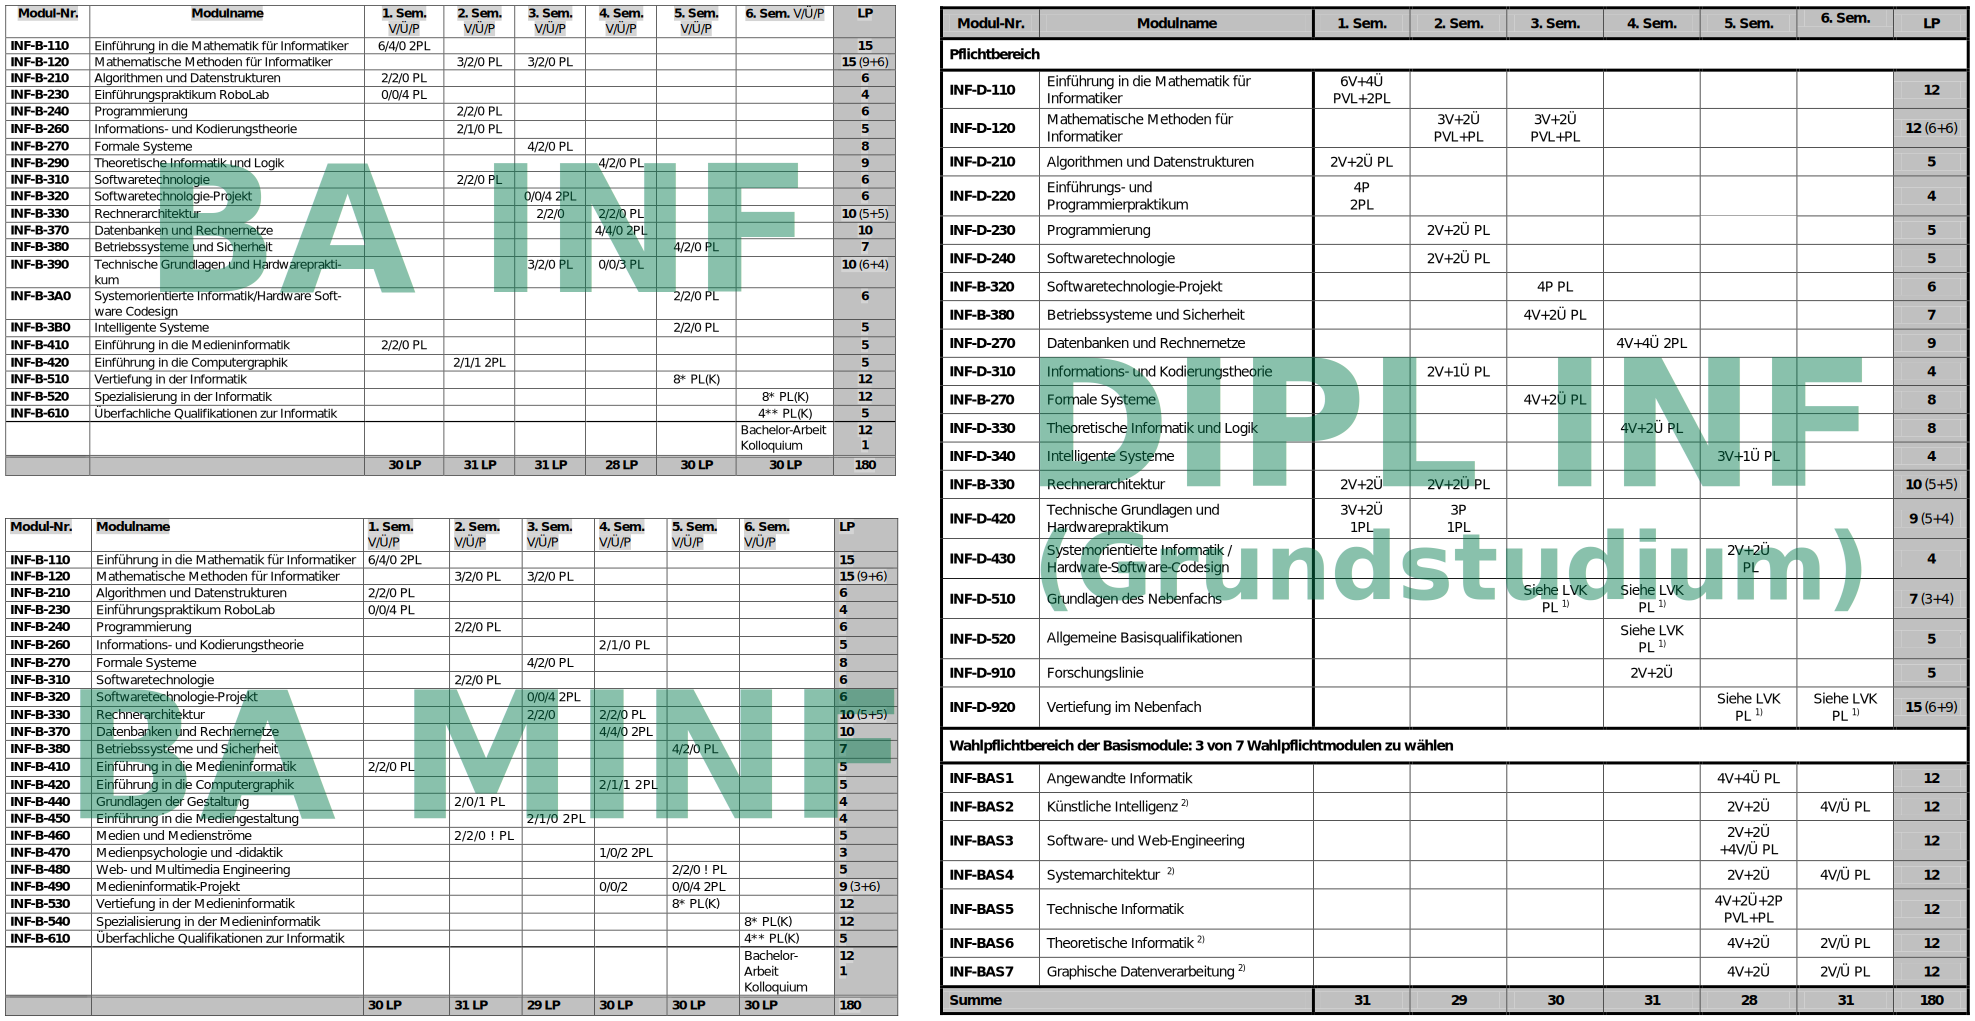
\includegraphics[width=\textwidth]{img/alle_studienablaufplaene.png}
	\caption*{\small \textit{Die Studienablaufpläne aller Studiengänge findest du in groß unter}~\link{https://tu-dresden.de/ing/informatik/studium/studienangebot}.}
\end{figure}

\minisec{Vorlesung}

In der Vorlesung wird der Stoff vermittelt, der schlussendlich in der Prüfung abgefragt wird. 
Es ist also sinnvoll, die Vorlesung aktiv zu verfolgen und sie ggf. vor- und nachzubereiten. 
Nicht ratsam ist es, erst vor der Prüfung den ganzen Stoff aufzuholen, da die Stoffmenge in der Regel sehr groß ist und es also unnötig mehr Stress in der Prüfungsphase bedeuten würde. \\
Besonders am Anfang deines Studium ist die Zahl der Zuhörer einer Vorlesung im dreistelligen Bereich. 
Daran gewöhnt man sich aber in der Regel schnell.
Je mehr Leute aber in einer Vorlesung sitzen, desto Wahrscheinlicher ist es, dass jemand an einer Stelle in der Vorlesung nicht mitkommt. 
Das kann jedem mal passieren.
Falls du also dieser jemand sein solltest, habe keine falsche Scheu, den Dozierenden eine Frage zu stellen, um die Unklarheiten zu beseitigen. 
Aktive Beteildigung in der Vorlesung ist immer gerne gesehen bei den Dozierenden.
Und ja, auch wenn es eine Verständnisfrage ist. 
Wahrscheinlich freut sich dann auch der ein oder andere Kommilitone von dir, der dieselbe Frage, aber nicht den Mut hatte zu fragen. \\
Welche Vorlesung du in welchem Semester besuchen solltest, findest du im jeweiligen Studienablaufplan deines Studiengangs
(Bachelor Informatik~\link{https://www.verw.tu-dresden.de/AmtBek/PDF-Dateien/2016-06/11soBA24.04.2016.pdf}, Bachelor Medieninformatik~\link{https://www.verw.tu-dresden.de/AmtBek/PDF-Dateien/2016-06/11soBAMI24.04.2016.pdf}, Diplom Informatik~\link{https://tu-dresden.de/die_tu_dresden/fakultaeten/fakultaet_informatik/studium/dateien/studien_und_pruefungsordnungen/dipl_inf_so_app1_de.pdf}) oder im Vorlesungsverzeichnis auf der Seite der Fakultät~\link{https://tu-dresden.de/ing/informatik/studium/lehre}. 


\minisec{Übung}

Übungen werden zu fast allen Vorlesungen angeboten und dienen dazu, Aufgaben zum aktuellen Vorlesungsstoff zu bearbeiten. Klausuren orientieren sich häufig an den Übungsaufgaben, deshalb solltest du die Übungen
regelmäßig besuchen. Die Übungen werden meistens von Studenten aus höheren Semestern oder von Lehrstuhlmitarbeitern gehalten, nicht vom Professor.
Das hat auch den Vorteil, dass man bekanntlich viele Dinge besser versteht, wenn man sie noch einmal aus einem anderen Mund erklärt bekommt.
Die jeweils aktuellen Übungsaufgaben findest du auf der Seite des jeweiligen Dozenten, oft unter den Stichworten Teaching oder Lehre.
Es wird erwartet, dass du dir die Aufgaben bereits vor der Übung anschaust, um dann Lösungen oder Fragen zu diskutieren.


\minisec{Praktikum}

Das erste Praktikum erwartet dich bereits in der vorlesungsfreien Zeit des ersten Semesters -- plane deinen Urlaub also lieber nicht zu schnell!
Dort wirst du im Einführungspraktikum \textit{Robolab} dein Können unter Beweis stellen. Diplomer müssen zusätzlich noch das Strategiespielepraktikum absolvieren.
Ein ganzes Praktikumssemester ist nur für Diplomstudenten im 7. Semester Pflicht.
Natürlich ist es trotzdem empfehlenswert, Praktika bei echten Firmen außerhalb der Fakultät in den Semesterferien zu machen, das steigert nicht nur deine Jobchancen,
sondern zeigt dir auch, ob deine Studienwahl tatsächlich die Richtige war.

\refstepcounter{dummy}\label{sec:pruefungen}
\minisec{Prüfungen}
Direkt an die Vorlesungszeit schließt die Prüfungszeit an – die wohl stressigste Zeit im Leben eines Studenten.
Die genauen Prüfungstermine findest du für das Wintersemester meist etwa Anfang Januar auf der Homepage der Fakultät~\link{https://tu-dresden.de/ing/informatik/studium/news} oder direkt beim Prüfungsamt~\link{https://tu-dresden.de/ing/informatik/studium/pruefungsorganisation}.
Im Laufe des Semesters hast du die Gelegenheit, dich dafür (innerhalb der Einschreibefrist) über jExam einzuschreiben.
Dort hast du auch die Möglichkeit, dich bis zu drei \emph{Werk}tage vor der Prüfung wieder auszutragen. Du kannst die Prüfung auch in einem späteren Semester schreiben. Das sollte aber natürlich nicht zum Regelfall werden. Für mündliche und sonstige Prüfungen gilt eine Abmeldefrist von 14 Tagen.
Solltest du aufgrund eines Rücktritts innerhalb der Frist oder einer plötzlichen Erkrankung von der Prüfung ausscheiden, kannst du dich auf der Seite des Prüfungsamtes informieren,
welche Nachweise (Atteste) du im Prüfungsamt innerhalb welcher Frist einreichen musst~\link{https://tu-dresden.de/ing/informatik/studium/pruefungsorganisation/pruefungen/abmelden-ruecktritt-krankheit}.
Prüfungen werden mit Noten bewertet, wobei alle mit besser als 5.0 bewerteten Prüfungen als bestanden gelten und nicht wiederholt werden können.
Noten Schlechter als 5.0 gibt es nicht.
Die 5.0 ist damit die einzige Chance, eine Prüfung nicht zu bestehen.
Hast du das erst einmal geschafft, gibt es die Möglichkeit, die Prüfung innerhalb von zwei Semestern zu wiederholen.
Nach dem zweiten nicht geglückten Prüfungsversuch hast du nur noch ein Semester Zeit bis der dritte erfolgen muss.
Erst wenn du das dritte Mal die Klausur nicht bestanden hast (also die zweite Wiederholungsklausur), wirst du exmatrikuliert.
Genauere Informationen zu dieser Thematik findest du stets in der Prüfungs- bzw.\ der Studienordnung, die du dir unbedingt mal angeschaut haben solltest.
Deine erste Matheprüfung erwartet dich übrigens bereits im Dezember: die sogenannte Nikolausklausur.

\begin{figure}
	\begin{tikzpicture}
		\draw (0,0) rectangle (4,-5);
		\draw (0,0) [fill=black] rectangle (4, -.5);
		\node at (2,0) [below] {\textcolor{white}{Die meisten Module:}};
		\draw (0,-.5) [fill=gray!40] rectangle (4,-1);
		\node at (2,-.5) [below] {bspw. AuD};
		\draw (0,-.5) -- (4,-.5);
		\node (v1) [draw] at (2,-1.6) {Vorlesung};
		\node (u1) [draw] at (2,-2.7) {Übung};
		\draw (0,-3.5) -- (4,-3.5);
		\node (p1) [draw] at (2,-4.3) {Prüfung};

		\draw (5,0) rectangle (12, -5);
		\draw (5,0) [fill=black] rectangle (12, -.5);
		\node at (8.5,0) [below] {\textcolor{white}{Spezialfall Mathe im 1. Semester:}};
		\draw (5,-.5) -- (12,-.5);
		\node (pvl) [rectangle,draw,font=\scriptsize] at (8.5,-3.3) [above]{Hausaufgaben};
		\draw (8.5,-.5) -- (pvl);
		\draw (5,-.5) [fill=gray!40] rectangle (8.5,-1);
		\node at (6.75,-.5) [below] {LAG};
		\draw (8.5,-.5) [fill=gray!40] rectangle (12,-1);
		\node at (10.25,-.5) [below] {DIS};
		\draw (5,-1) -- (12, -1);
		\node (v2) [draw] at (6.6,-1.6) {Vorlesung};
		\node (u2) [draw] at (6.1,-2.7) {Übung};
		\node (v3) [draw] at (10.1,-1.6) {Vorlesung};
		\node (u3) [draw] at (10.9,-2.7) {Übung};
		\draw (5,-3.3) -- (12,-3.3);
    \node (p2) [draw] at (7.35,-4) {\enquote{Nikolausprüfung}};
		\node (p3) [draw] at (10.7,-4.4) {Prüfung};
		%\draw[->,thick] (pvl) -- (p3);
	\end{tikzpicture}
\end{figure}

\newpage

\minisec{Leistungsnachweis}

Bei manchen Prüfungen erhältst du neben der Note einen Leistungsnachweis (oder kurz: Schein).
Dazu zählen unter anderem die Sprachkurse, die Forschungslinie und z.T. Nebenfachprüfungen. Diese Scheine brauchst du, um dir diese Leistungen im Prüfungsamt anrechnen lassen zu können.

\refstepcounter{dummy}\label{sec:sprachausbildung}
\minisec{Sprachausbildung}

Es werden an der TU Dresden Kurse für fast alle möglichen (und unmöglichen) Sprachen angeboten.
Zu diesem Zweck gibt es zwei Zentren für die Sprachausbildung: Das \enquote{Lehrzentrum Sprachen und Kulturen} (LSK) und \enquote{TUD Institute of Advanced Studies} (TUDIAS).
Das Sprachangebot der beiden Einrichtungen ähnelt sich sehr stark.
Du hast für diverse Sprachkurse ein Budget an Semesterwochenstunden (insgesamt 10 SWS), die du ausgeben kannst, wie du willst.
Für dein Studium zum Bachelor der (Medien-)Informatik sind Sprachkurse generell optional, aber auf jeden Fall empfehlenswert.
Für Diplomstudenten sind 2 Semester Englisch im Laufe des Studiums Pflicht.
Studierst du allerdings Bachelor Informatik und möchtest danach mit dem Master Informatik an der TU Dresden weitermachen, wirst du für den Master das Sprachniveau B2 in Englisch nachweisen müssen,
also kann es sich auch für dich anbieten, die entsprechenden Sprachkurse zu besuchen.
Die Einschreibung für einen Sprachkurs erfolgt online~\link{https://sprachausbildung.tu-dresden.de} mit deinem ZIH-Login.
Sobald die Kurse freigeschaltet sind, solltest du dich jedoch stark beeilen, denn die beliebten Kurse sind meist innerhalb weniger Minuten voll.
Weitere Infos findest du unter~\link{https://tu-dresden.de/lsk}~und~\link{https://www.tudias.de/}.

\vfill
\begin{center}
  \includegraphics[trim={0 4cm 0 0}, clip, width=\linewidth]{img/ese2013/foyer.jpg}
\end{center}

\minisec{Schreibberatung}
Das Schreibzentrum der TU Dresden~\link{https://www.facebook.com/SchreibzentrumTUD} ist ein Kooperationsprojekt für Studierende und Lehrende vom Zentrum für Weiterbildung und dem Career Service. Es bietet Unterstützung, Methoden und Ideen zum Thema \enquote{wissenschaftliches Schreiben}.
Du kannst mit deinen Schreibprojekten aller Art (Beleg, Seminararbeit, Abschlussarbeit, etc.) entweder in die offene Schreibsprechstunde am SCS ServicePoint der SLUB kommen oder einen individuellen Termin per E-Mail~\link{mailto:Schreibzentrum@mailbox.tu-dresden.de} vereinbaren.
Dabei spielt es keine Rolle, wie weit die Arbeit bereits ist, ob man also noch ganz am Anfang steht oder kurz vor der Abgabe.
Auch muss kein konkretes Problem vorliegen, sondern intuitive Anliegen zur Arbeit können ebenfalls geschildert werden.

Die Schreibberatung unterstützt bei Fragen zum Schreibprozess -- von der Themenfindung, über die Gliederung bis hin zur Abgabe der fertigen Arbeit.
Ausgebildete studentische Schreibtutorinnen und Schreibtutoren unterstützen dich mit vielfältigen Schreibmethoden und Techniken.
Inhaltliche Tipps oder Hilfestellungen können dir dabei nicht gegeben werden.
Auch liest die Schreibberatung keine Texte Korrektur; allerdings kannst du exemplarisch Textfeedback auf Textauszüge bekommen.
Das Angebot ist selbstverständlich kostenlos.

\minisec{Stipendien}

Neben dem BAföG sind auch Stipendien eine gern genutzte Möglichkeit der Studienfinanzierung.

Viele Stipendien werden von den 13 überwiegend staatlich finanzierten Begabtenförderungswerken vergeben, die sich hinsichtlich ihres weltanschaulichen, religiösen oder politischen Profils unterscheiden.
Oftmals werden Studierende aufgrund guter Leistungen von Schulen, Prüfungsämtern oder Hochschullehrern direkt vorgeschlagen.
Bei vielen Werken sind aber auch Selbstbewerbungen möglich.
Für die Aufnahme muss man keineswegs ein Überflieger sein.

Im Auswahlprozess können gesellschaftliches oder soziales Engagement eine ebenso wichtige Rolle spielen.
Die Stipendien werden in Anlehnung an das BAföG abhängig vom eigenen Einkommen und Vermögen sowie vom Einkommen der Eltern berechnet.
Zusätzlich erhalten die Stipendiaten eine monatliche Studienkostenpauschale in Höhe von 300 Euro.
Im Gegensatz zum BAföG müssen die Stipendien jedoch nicht zurückgezahlt werden.
Neben der finanziellen Förderung bieten alle Werke eine umfangreiche ideelle Förderung in Form von Sprachkursen, Exkursionen und Akademien.

Ebenso bekannt ist das Deutschlandstipendium, welches zur Hälfte von privaten Geldgebern finanziert wird.
Die finanzielle Förderung erfolgt unabhängig vom eigenen Einkommen oder dem der Eltern und beläuft sich auf 300 Euro monatlich.
Das Deutschlandstipendium wird nicht auf das BAföG angerechnet und muss ebenfalls nicht zurückgezahlt werden.
Bewerbungen werden jeweils im Juli direkt vom Zentrum für Weiterbildung der TU Dresden~\link{https://tu-dresden.de/deutschlandstipendium} entgegengenommen.

Es gibt noch viele weitere Organisationen, deren Förderung überwiegend privat finanziert wird. Diese vergeben jedoch oft nur wenige Vollstipendien oder beschränken die Förderung auf geringere Sach- oder Geldleistungen.
Einen Überblick über die Vielzahl an Förderungsmöglichkeiten kann man mithilfe der Stipendiendatenbank des BMBF~\link{https://www.stipendienlotse.de} erhalten.

\begin{figure}[b]
	\centering
	\includegraphics[width=\textwidth, keepaspectratio]{img/xkcd/zealous_autoconfig.png}
	\caption*{{\small \textit{I hear this is an option in the latest Ubuntu release. (https://xkcd.com/416)}}}
\end{figure}

\minisec{Hochschulgruppen}
\label{sec:hsg}

Lernen und feiern reicht dir nicht?
Such dir eine Hochschulgruppe!
Dort findest du ehrenamtlich engagierte Studierende, die aktiv das Leben auf
dem Campus mitgestalten wollen.
Und je nachdem was du suchst, wirst du auch Diskussionen, die Möglichkeit anderen zu helfen, neue Erfahrungen, interessante Leute und vieles mehr finden können.

Thematisch ist für jeden etwas dabei.
So gibt es Hochschulgruppen mit politischem und gesellschaftlichem Engagement.
Andere sind interessiert an der Gestaltung kultureller Vielfalt in Dresden.
Natürlich sind aber auch technisch orientierte Hochschulgruppen vertreten.
Schau dich einfach mal hier~\link{https://www.stura.tu-dresden.de/hochschulgruppen} um und melde dich direkt bei einer Hochschulgruppe deiner Wahl.
Vielleicht ist ja was für dich dabei.

\minisec{Auslandsaufenthalte}

Bei akutem Auslandswunsch oder studienbegleitendem Internationalisierungsdrang fragen Sie bitte das Auslandsamt der Uni oder Ihren Professor des Vertrauens.
Auslandsaufenthalte können Nebenwirkungen hervorrufen.
Über diese können Sie sich bei Kommilitonen erkundigen.

Im Verlaufe deines Studiums werden dich immer wieder Leute fragen, ob du nicht ein oder zwei Semester im Ausland verbringen möchtest.
Nun magst du dich als unschuldiger Erstsemester fragen, warum denn das und wieso kommt ihr jetzt schon damit an?
Die Antwort ist einfach:
Zum einen kannst du direkt deine Sprachkenntnisse verbessern, Kontakte knüpfen und neue Kulturen erleben -- Eine willkommene Abwechslung, um den Kopf frei zu bekommen nach den anstrengenden Semestern. Es werden neue Perspektiven vermittelt, sowohl akademisch als auch fachlich. Außerdem hilft es dir bei der Entwicklung deiner Softskills wie Selbstständigkeit, Toleranz und Anpassungsfähigkeit (um nur einige zu nennen). Alles Dinge, die dir später weiterhelfen werden und für die du später dankbar sein wirst.
Kurz und knapp gesagt ein Auslandsaufenthalt ist nützlich, erfordert aber etwas Planung.
Deshalb ist es von Vorteil sich möglichst früh zu informieren.
Für Infos und bei Fragen kannst du dich an das Akademische Auslandsamt (AAA) der TU~\link{https://tu-dresden.de/studium/im-studium/beratung-und-service/akademisches-auslandsamt} wenden und auf den Seiten der Fakultät~\link{https://tu-dresden.de/ing/informatik/studium/internationales/outgoing} informieren.
Wenn man mutig ist, kann man sogar Professoren direkt fragen, ob sie Kontakte zu anderen Unis oder Unternehmen haben.
Es liegt an dir, wie erfolgreich dein Auslandsaufenthalt wird.
Ob beim Streicheln von Robben vor Neufundland oder beim Scrum-Meeting im Silicon Valley, es gibt eine Menge Angebote, die auf dich warten!

% \begin{figure}[b!]
% 	\centering
% 	\includegraphics[width=0.9\linewidth]{img/ese2014/einschreibung.jpg}
% \end{figure}%

\minisec{Urlaubssemester}
Es gibt eine ganze Reihe von Gründen, die dich daran hindern können, dein Studium an der TU ordnungsgemäß weiterzuführen.
Klassische Gründe sind schwere Erkrankungen, längere Praktika, Auslandsaufenthalte oder (unverhoffter) Nachwuchs, um den du dich kümmern musst.
In solchen Fällen kannst du dich von deinem Studium beurlauben lassen, um dich voll und ganz auf den Urlaubsgrund zu konzentrieren.
Während eines Urlaubssemesters bist du von der Pflicht befreit, Prüfungen ablegen zu müssen, genießt aber weiterhin alle Vorteile des Studierendendaseins.
Andererseits hast du in dieser Zeit meist auch keinen Anspruch auf BAföG- oder Kindergeld-Zahlungen, also plane das nicht unbedingt bei deinen Einkünften ein.

Solltest du ein Auslandsstudium machen und ein paar Semester in fernen Landen verweilen, kannst du dir danach erbrachte Leistungen und Prüfungen hier anrechnen lassen.
Einziger Fallstrick dabei: Wenn du genügend Leistungspunkte einbringst, wirst du trotzdem ein Fachsemester hochgestuft, aber da kann dir die Studienfachberatung weiterhelfen.

Beantragen kannst du ein Urlaubssemester beim Immatrikulationsamt~\link{https://tu-dresden.de/imma/} während der Rückmeldefrist für das nächste Semester.
Wie genau das geht und weitere Informationen findest du unter~\link{https://tu-dresden.de/studium/im-studium/studienorganisation/beurlaubung}.

\addchap{Modulübersicht}

Ein (M) kennzeichnet ein Modul nur für Medieninformatiker, ein (I) jeweils Module für Informatiker und ein (D) für Diplominformatiker.

\minisec{{\Large\ \\ 1. Semester\\\ }}

\textbf{\menu[,]{I, M, D, Einführung in die Mathematik für Informatiker\,}}\\
Ihr kennt euch mit Matrizen aus?
Dann wisst ihr auch was mit den Begriffen Determinante, Diagonalisierbarkeit, Skalarprodukt und Lösung eines homogenen linearen Gleichungssystems anzufangen - wenn nicht, dann lernt ihr es hier von der Pike an.
Außerdem wird in der Diskreten Mathematik das Mal und Plus quasi neu definiert und ihr lernt ein wenig anders zu denken.

\textbf{\menu[,]{I, M, D, Algorithmen und Datenstrukturen\,}} \\
Was kommt zuerst?
5 oder 3?
Solche Fragen werden euch in Algorithmen und Datenstrukturen beschäftigen während ihr Quicksort, Heapsort und Konsorten lernt.
% Der Wortwitz gefällt mir...
Weiter werdet ihr euch als Gärtner versuchen indem ihr AVL- und andere Bäume wachsen lasst.
Dabei werdet ihr Bekanntschaft mit der Programmiersprache C machen.

\textbf{\menu[,]{I, M, D, Einführungspraktikum\,}} \\
Ihr habt schon immer gerne mit Lego gespielt?
Dann wird euch dieses Praktikum, welches in der vorlesungsfreien Zeit stattfindet, gefallen.
Ihr dürft euch im Team daran machen einen selbst konstruierten Roboter in C beizubringen, wie er sich in einem Labyrinth alleine zurechtfindet.
Dabei, und im anschließenden Wettbewerb, kommt der Spaß nicht zu knapp.
Für Diplomstudenten gibt es zusätzlich ein einwöchiges Einzelprojekt, bei dem man zeigen kann, was man in C oder wahlweise C++ drauf hat. Alternativ kann das Strategiespielepraktikum auch auf das Sommersemester verschoben werden.
Im letzten Jahr war eine KI für bekannte Brettspiele gefragt.

\textbf{\menu[,]{I, M, Einführung in die Medieninformatik\,}} \\
Anfangs erfolgt eine Darstellung des menschlichen Wahrnehmungssystems, Aspekte der Wahrnehmungspsychologie und der Softwareergonomie.
Dann werden Eigenschaften der Information und Datenformate anhand der Medien Text, Bild, Audio und Video dargestellt.
Im Bereich Text und Bild werden die entsprechenden Dokumentenformate des Internet (HTML und SVG) besprochen.
Ein weiterer Teil der Lehrveranstaltung gibt einen Überblick zur Dokumentenverarbeitung mittels XML-Techniken.
Die Praxis wird in den Gruppenübungen erworben und in kleinen Teams ein Projekt erarbeitet.

\textbf{\menu[,]{D, Technische Grundlagen und Hardwarepraktikum\,}} \\
siehe INF-B-390, 3. Semester.

\textbf{\menu[,]{D, Rechnerarchitektur\,}} \\
siehe INF-B-330, 3. Semester.

\minisec{{\Large\ \\ 2. Semester\\\ }}

\textbf{\menu[,]{I, M, D, Mathematische Methoden für Informatiker\,}} \\
Nachdem der Abistoff wieder und viel tiefer als vorher sitzt, geht es in den nächsten zwei Semestern in neue Bereiche der Mathematik.
Anfangs werden die verschiedenen Typen algebraischer Strukturen (das sind Mengen von beliebigen Symbolen und darauf erklärte Rechenoperationen) untersucht.
Es folgen Vektoren, Matrizen und mathematische Körper.
Dann kommt ein Sprung vom Diskreten zum Kontinuierlichen.
So langweilig wie in der Schule ist Analysis nämlich gar nicht, die gibt es auch in der Ausführung mit mehreren Veränderlichen.
Das Ganze gipfelt in der Einführung von Differentialgleichungen.
Gegen Schluss wendet man sich erneut den Polynomen zu.
Dabei werden zunächst effiziente Näherungsverfahren behandelt.
Später folgt dann ein kurzer Ausflug in die Stochastik.

\textbf{\menu[,]{I, M, D, Programmierung\,}} \\
Dass Programmiersprachen nicht auf Bäumen wachsen, wusstet ihr wahrscheinlich schon, doch dass sie strengen mathematischen Regeln folgen, lernt ihr hier.
Am Beispiel eines Teils der Programmiersprache C wird zunächst die Syntax mit Hilfe von Grammatiken definiert.
Kurz darauf kommt ihr in den Kontakt mit der funktionalen Programmiersprache Haskell.
Durch viele hübsche, rekursiv verschachtelte Abbildungen wird dann die Semantik festgelegt, d.h. die Wirkung, die so ein Programm auf einer (abstrakten) Rechenmaschine hat.
Hier wird auch vermittelt, wie man die Korrektheit eines Programmstückes "wasserdicht", d.h. formal logisch beweisen kann.

\textbf{\menu[,]{I, M, D, Informations- und Kodierungstheorie\,}} \\
Was Informationen eigentlich sind, was sie ausmacht, wird euch hier beschäftigen.
In dieser Lehrveranstaltung werdet ihr einen Einstieg in ein sehr interessantes und komplexes Fachgebiet erhalten.
Im Mittelpunkt steht am Anfang wie man Informationen darstellen und speichern kann.
Etwas später wird erklärt, warum und wie die Informationen mittels Kodierung geschützt werden, damit sie bei euch sicher ankommen, wenn sie unterwegs Störungen und Manipulationen ausgesetzt sind.
Dabei wird euch euer in der Mathematik erworbenes Wissen von Nutzen sein.

\textbf{\menu[,]{I, M, D, Softwaretechnologie\,}} \\
Software zu entwickeln ist eine Kunst, das werdet ihr spätestens nach diesem Modul erkennen.
Um diese Kunstfertigkeit an den Tag legen zu können bedarf es einiger Handwerkszeuge, welche ihr hier mit auf den Weg bekommt.
So werden euch moderne Konzepte am Beispiel von Java und Entwurfsverfahren zusammen mit professioneller Dokumentation näher gebracht.
Damit wird dann der Grundstein für das Projekt im dritten Semester gelegt, bei dem man sich Lorbeeren im Projektmanagement und als Entwickler verdienen kann.

\textbf{\menu[,]{I, M, Einführung in die Computergraphik\,}} \\
Es geht um den Aufbau von Grafiksystemen, Farbräumen, Rastergraphiken und deren Anwendungen.
Bestehende Probleme, wie Aliasing und Artefakte sind mit von der Partie, sowie ihre algorithmischen Lösungen.
Als Programmiersprache für die Übungsaufgaben wird C++ genutzt.

\textbf{\menu[,]{D, Technische Grundlagen und Hardwarepraktikum\,}} \\
Fortsetzung aus dem 1. Semester.

\textbf{\menu[,]{D, Rechnerarchitektur\,}} \\
Fortsetzung aus dem 1. Semester.

\minisec{{\Large\ \\ 3. Semester\\\ }}

\textbf{\menu[,]{I, M, D, Mathematische Methoden für Informatiker\,}} \\
Fortsetzung aus dem 2. Semester.

\textbf{\menu[,]{I, M, D, Formale Systeme\,}} \\
Wahr?
Und oder falsch?
Was falsch ist wird, wenn es falsch falsch ist, wahr?
Logisch!
Neben der Aussagenlogik vermittelt das Modul die Grundlagen formaler Sprachen.
Es folgen Gedanken zu maschinellen Berechenbarkeit und zur Automatentheorie.
Turing lässt grüßen.

\textbf{\menu[,]{I, M, D, Softwaretechnologie-Projekt\,}} \\
Das Projekt nimmt den größten Teil des dritten Semesters ein.
Hier muss man sein Wissen aus der Lehrveranstaltung "Softwaretechnologie" in die Tat umsetzen.
In einem fünfköpfigen Team hat man die Aufgabe, eine Anwendung von vorn bis hinten fertig zu stellen.
Dabei muss man häufig Rücksprache mit den "Kunden" halten.
Abgeschlossen wird das Modul mit einer Präsentation des fertigen Produkts vor dem Kunden und den Verantwortlichen des Moduls.
Am Ende habt ihr dann einen Eindruck, wie die Arbeit eines Informatikers aussehen kann.

\textbf{\menu[,]{I, M, Rechnerarchitektur\,}} \\
Hier geht es um die Grundbausteine eines Computers:
Speicher, Bussysteme, Rechen- und Steuerwerk.
Außerdem erhält man eine Einführung in Assembler, das Pipelining-Prinzip und damit auftretende Probleme.
Schließlich wird noch diskutiert, mit welchen Methoden man heutige Rechnerarchitekturen beschleunigen kann und parallele Architekturen nutzen kann.

\textbf{\menu[,]{I, Technische Grundlagen und Hardwarepraktikum\,}} \\
Wer schon immer mal wissen wollte, was die Strömlinge im häuslichen Rechner eigentlich so alles durchmachen müssen, bekommt das genau vermittelt.
Anfangs werden Transistor-, Dioden- und Operationsverstärkerschaltungen betrachtet.
Darauf aufbauend geht es über Verknüpfungsglieder und komplexe Schaltungen.

\textbf{\menu[,]{M, Grundlagen der Gestaltung\,}} \\
Die Vorlesung beginnt mit Begriffsdefinitionen sowie allgemeinen Gestaltungsprinzipien und erläutert diese.
Dabei beschränkt sich die Veranstaltung bewusst auf zweidimensionale Bereiche.
Formkategorien, Kontrastbildung und Farblehre bilden die Schwerpunkte.
Die begleitenden Übungen sollen einen Einblick in die Materie vermitteln und die Sensibilität der Studierenden durch handwerkliches Arbeiten wecken.

\textbf{\menu[,]{D, Grundlagen des Nebenfachs\,}} \\
Je nachdem, was ihr euch als Nebenfach wählt, beschäftigt ihr euch hier mit Themen die nur im entfernten Sinne mit Informatik zusammenhängen.
Über den Tellerrand schauen und andere Welten kennenlernen ist das Motto.

\textbf{\menu[,]{D, Betriebssysteme und Sicherheit\,}} \\
siehe INF-B-380, 5. Semester.

\minisec{{\Large\ \\ 4. Semester\\\ }}

\textbf{\menu[,]{I, D, Theoretische Informatik und Logik\,}} \\
Die Fortsetzung der Formalen Systeme.
Es folgen weitere Betrachtung zur Korrektheit und Terminierung von Algorithmen und der notwendige Aufwand in Form von Zeit und Platzbedarf.
Ein Abstecher in die Prädikatenlogik und Logikprogrammierung rundet das Modul ab.

\textbf{\menu[,]{I, M, Rechnerarchitektur\,}} \\
Fortsetzung aus dem 3. Semester.

\textbf{\menu[,]{I, M, D, Datenbanken und Rechnernetze\,}} \\
In dieser Lehrveranstaltung lernt man zuerst Methoden zur effizienten Datenspeicherung kennen.
Danach wird die Fähigkeit vermittelt, selbst komplexe relationale Datenbanken zu konzipieren und zu erstellen.
Auch werden Rechnernetze behandelt.
Angefangen mit dem Funktionsprinzip von Modem und Netzwerkkarte erhält man einen kurzen Überblick über moderne Kommunikations- und Vermittlungsprotokolle.
Auch der Sektor Mobilkommunikation und die dabei auftretenden Schwierigkeiten werden kurz beleuchtet.

\textbf{\menu[,]{I, Technische Grundlagen und Hardwarepraktikum\,}} \\
Fortsetzung aus dem 3. Semester.

\textbf{\menu[,]{M, Einführung in die Mediengestaltung\,}} \\
Die Vorlesung vermittelt die Grundzüge des multimedialen Gestaltens unter Gesichtspunkten der Entwicklung der einzelnen Richtungen (Film, Internet) mit Bezug auf die gestalterischen Änderungen in den vergangenen Jahrhunderten (Buch).
Außerdem wird in die Metaphernbildung eingeführt und einige Gastdozenten aus der Praxis vermitteln ihre Sicht auf die Mediengestaltung.

\textbf{\menu[,]{M, Medien und Medienströme\,}} \\
Hier wird Wissen zu Medien, deren Kompression und Bearbeitung vermittelt.
Die Anwendung verschiedener Werkzeuge zur Erzeugung von Medien und deren Charakteristika sind ebenfalls Gegenstand dieser Lehrveranstaltung.

\textbf{\menu[,]{M, Medienpsychologie und -didaktik\,}}
Mediendidaktik ist die "Kunst des Lehrens".
Hier werden die Fragen beantwortet:
Was ist Bildung?
Wie verläuft sie?
Wie lässt sie sich vervollkommnen?
Man erfährt etwas über die Entwicklung von Lehrmethoden.
Im parallel stattfindenden Praktikum wird das Gelernte gleich praktisch bei der Erstellung eines Lernprogramms angewandt.

\textbf{\menu[,]{M, Komplexpraktikum\,}} \\
Das große Highlight für Medieninformatiker im Bachelor.
In kleineren Gruppen soll ein mobiles Spiel, eine Internet-Seite, ein Film oder Multimediales realisiert werden.
Abgesehen von der Aufgabenstellung sind der Fantasie quasi keine Grenzen gesetzt.
Es geht um harte Arbeit, Teamgeist und das Ernten der wohlverdienten Lorbeeren.

\textbf{\menu[,]{D, Forschungslinie\,}} \\
Hier bekommt ihr einen Überblick über aktuelle Forschungsthemen und bekommt vermittelt, wie man forschungsorientiert arbeitet.
Dieses Modul hilft, später die richtige Vertiefung zu wählen.

\textbf{\menu[,]{D, Grundlagen des Nebenfachs\,}} \\
Fortsetzung aus dem 3. Semester.

\textbf{\menu[,]{D, Allg. Basisqualifikationen\,}} \\
Englisch ist die einzig relevante Sprache in der Informatik.
Hier wird euch vermittelt, wie man sich fachlich auf Englisch ausdrückt.
Abgerundet wird das Modul durch eine Schulung eurer Vortragsfähigkeiten.

\minisec{{\Large\ \\ 5. Semester\\\ }}

\textbf{\menu[,]{I, M, Betriebssysteme und Sicherheit\,}} \\
Diese Lehrveranstaltung nimmt die dienstbaren Geister, die zwischen der Hardware und den bunten Anwendungen werkeln, unter die Lupe.
Warum kann man mit einem Rechner gleichzeitig einen Text schreiben, compilieren, ein Bild berechnen und Musik hören?
Wie werden meine Daten in Rechnersystemen geschützt?
Wieso stehen die hier auf dieses Unix?

\textbf{\menu[,]{I, D, Systemorientierte Informatik/ Hardware Software Codesign\,}} \\
Dieses Fachgebiet ist die Schnittstelle zwischen Rechnern und der industriellen Praxis, die von der Steuerung von Heizventilen bis zu Kraftwerken reicht.
Zunächst wird abstrahiert, was allen praktisch vorkommenden Systemen gemein ist, und es werden Modelle wie "System", "Signal" und "Regelkreis" erschaffen, mit denen sich dann rechnerisch umgehen lässt.
Hier wird man fit gemacht für die Analyse und Voraussage von Übertragungsverhalten und Reaktionen, die ein solches System bei einem bestimmten Input zeigen wird.
Daneben kommen auch Aspekte aus der Audio- und Videotechnik wie Digitalisierung und Filteralgorithmen nicht zu kurz.

\textbf{\menu[,]{I, D, Intelligente Systeme\,}} \\
In dieser Lehrveranstaltung geht es um künstliche Intelligenz.
Hier erlernt man Problemlösung, Wissensrepräsentation, Planung, Wahrnehmung und Sprachverstehen, mit Hilfe spezieller Algorithmen und Agenten.

\textbf{\menu[,]{M, Web- und Multimedia Engineering\,}} \\
Wie kann man Web mit heutiger Technik multimedial und interaktiv gestalten?
Wie nutze ich professionelle Entwicklungswerkzeuge und geeignete Sprachen, wie z.B. Java, um meine Vorstellung in das Ergebnis zu projizieren?
Dieses Modul hilft geeignete Methoden zu erlernen und Erfahrung bei der Anwendung zu sammeln.

\textbf{\menu[,]{M, Komplexpraktikum\,}} \\
Fortsetzung aus dem 4. Semester.

\textbf{\menu[,]{I, M, D, Vertiefung\,}} \\
Hier kann der Student aus einem Angebotskatalog geeignete Veranstaltungen wählen um seinen wissenschaftlichen Horizont zu vertiefen.
Die Möglichkeiten umfassen Vorlesungen, Übungen, Praktika, Projektbearbeitungen, Exkursionen, Proseminare, Tutorien und Sprachkurse.

\textbf{\menu[,]{D, Vertiefung im Nebenfach\,}} \\
Nachdem ihr euch die Grundlagen eures gewählten Nebenfachs angeeignet habt, wird es nun ernst und ihr steigt tiefer in die Materie ein.

\textbf{\menu[;]{D; Basismodul 1, 2 und 3\,}} \\
Hier wählt ihr unter sieben verschiedenen Themenkomplexen drei aus und beschäftigt euch mit ihnen.
Zur Wahl stehen Angewandte Informatik, Künstliche Intelligenz, Software- und Web-Engineering, Systemarchitektur, Technische Informatik, Theoretische Informatik, Graphische Datenverarbeitung.
Innerhalb dieser Richtungen stehen euch verschiedene Vorlesungen zur Auswahl.
Für mehr Infos müsst ihr die einschlägigen Webseiten und die Prüfungsordnung lesen.

\minisec{{\Large\ \\ 6. Semester\\\ }}

\textbf{\menu[,]{I, M, Vertiefung zur Bachelorarbeit\,}} \\
Weitere Vertiefung nach gleichem Muster wie im fünften Semester in Vorbereitung auf die Bachelorarbeit.

\textbf{\menu[,]{I, M, Allgemeine Qualifikation\,}} \\
In dieser Art Nebenfach orientiert sich der Student fächerübergreifend an Themen seines Interesse, um die fachspezifische Kompetenz zu entwickeln.
Auch hier können Veranstaltungen aus einem Katalog gewählt werden.

\textbf{\menu[,]{I, M, Bachelorarbeit und Kolloquium\,}} \\
Als krönenden Abschluss fertigt ihr die Bachelorarbeit zu einem von euch gewählten Thema an und verteidigt sie in einem Vortrag.

\textbf{\menu[,]{D, Vertiefung im Nebenfach\,}} \\
Fortsetzung aus dem 5. Semester.

\textbf{\menu[;]{D; Basismodul 1, 2 und 3\,}} \\
Fortsetzung aus dem 5. Semester.

\minisec{{\Large\ \\ 7. Semester\\\ }}

Angehende Diplominformatiker haben nach den sechs Semestern noch vier weitere vor sich.
Im siebten Semester werdet ihr ein Berufspraktikum absolvieren, im achten und neunten werdet ihr dann Module auswählen die euch interessieren und tiefer in die Abgründe des gewählten Themas hinabsteigen.
Im zehnten Semester wird ausschließlich die Diplomarbeit angefertigt und das war es dann schon!
So schnell kann es gehen.

\begin{figure}[h!]
\centering \includegraphics[width=\linewidth]{img/xkcd/exploits_of_a_mom.png}
\caption*{{\small \textit{Her daughter is named Help I'm trapped in a driver's license factory. (xkcd/327)}}}
\end{figure}

\thispagestyle{empty} %keine Seitenzahl
\AddToShipoutPicture*{\put(0,0){%
\parbox[b][\paperheight]{\paperwidth}{%
\vfill
\centering

\includegraphics[height=\pageheight, width=\pagewidth]{img/filmwerbung.pdf}
\vfill
}}}
\mbox{}

\addchap[Campusplan]{}
\thispagestyle{empty} %keine Seitenzahl
\AddToShipoutPicture*{\put(0,0){%
\parbox[b][\paperheight]{\paperwidth}{%
\vfill
\centering
\adjincludegraphics[height=\pageheight,keepaspectratio,trim={0 0 {.5\width} 0},clip]{img/campusplan_highlighted.pdf}%
\vfill
}}}
\mbox{}
\newpage
\thispagestyle{empty} %keine Seitenzahl
\AddToShipoutPicture*{\put(0,0){%
\parbox[b][\paperheight]{\paperwidth}{%
\vfill
\centering
\adjincludegraphics[height=\pageheight,keepaspectratio,trim={{.5\width} 0 0 0},clip]{img/campusplan_highlighted.pdf}%
\vfill
}}}
\mbox{}


\end{document}
